\chapter{Linear Algebra}
\label{chap:linear_algebra}
\markboth{Linear Algebra}{Linear Algebra}

\begin{remark}[Positioning of this chapter]\label{rem:linear_algebra_chapter_positioning}
Linear algebra is the mathematical theory that studies vector spaces, linear transformations and their algebraic structures. From the perspective of periodic mathematics, this chapter systematically establishes the foundational theory of linear algebra, focusing on the invariant subspace decomposition of linear transformations, the eigenvalue problem, and the profound connections between the spectral theorem and periodic structures. The central aim of this chapter is to provide a rigorous mathematical language for the analysis of linear systems.

This chapter is built on the foundations of the preceding chapters. Among them, the `Operations and Periodicity' chapter established the logical chain conservation law---symmetry---closed orbit---period; the `Number Systems' chapter established the correspondence between extensions of number systems and types of periodicity; the `Scalars and Vectors' chapter established the algebraic realisation of the three basic transformations at the level of vectors; and the `Functions and Limits' chapter established the unified framework direction---trend---convolution. This chapter systematically gathers these results into finite-dimensional vector spaces, revealing how the core theorems of linear algebra---the spectral theorem, the singular value decomposition and the classification of matrix groups---are the algebraic realisation of the three basic operators (gradient, divergence, curl).

The core work of this chapter lies in:
\begin{enumerate}[label=(\arabic*)]
    \item \textbf{Invariant subspaces and periodic orbits}: the invariant subspaces of a linear transformation correspond to the closed orbits of a dynamical system---evolution on a one-dimensional invariant subspace is a pure translation period, whilst rotation on a two-dimensional invariant subspace is a pure rotation period.
    \item \textbf{Eigenvalue decomposition and frequency spectrum}: the eigenvalue decomposition diagonalises a linear transformation into a direct sum of independent one-dimensional invariant subspaces. Each eigenvalue corresponds to a characteristic frequency, and each eigenvector corresponds to an epicycle component.
    \item \textbf{Spectral theorem and conservation law}: the spectral theorems for self-adjoint and unitary operators are respectively the formulation in linear algebra of the gradient (symmetry centre $0$) (real eigenvalues, pure translation) and of the curl (symmetry centre $i$) (eigenvalues of modulus $1$, pure rotation). The spectral decomposition is the realisation of the conservation law at the level of operators.
    \item \textbf{Matrix groups and symmetry}: the orthogonal group, the unitary group and the symplectic group correspond in periodic mathematics respectively to the matrix realisations of the three symmetry groups---translation ($0$-symmetry), rotation ($i$-symmetry) and scaling ($1$-symmetry).
\end{enumerate}

\textbf{Guide to the seven themes of this chapter}: translation---translation matrices and cyclic shifts (stretching/compression of real eigenvalues, DFT diagonalisation of circulant matrices); scaling---diagonal scaling and singular values (the diagonal matrix $\operatorname{diag}(\lambda_i)$, the $\boldsymbol{\Sigma}$ of the SVD, and volume scaling measured by the determinant); rotation---orthogonal and unitary matrices (eigenvalues of modulus $1$, plane rotations, the isometric action of $O(n)/U(n)$); conservation---the Frobenius norm, the determinant and the rank (conservation of dimension, energy conservation of $\sum_i \sigma_i^2$); symmetry---the matrix groups $O(n)/U(n)/Sp(2n)$ (matrix realisations of $0$-symmetry, $i$-symmetry and $1$-symmetry); closure---finite-order periodic solutions satisfying $\lambda^p = 1$ (eigenvalues lying on roots of unity, the cyclic structure of $C_p$); period---the periodic structure of linear systems (the four types of motion in the spectral decomposition, iterative convergence and steady states).
\end{remark}

\begin{figure}[htbp]
\centering
\begin{tikzpicture}[
  font=\small,
  obj/.style={draw, rounded corners, fill=blue!8, minimum width=2.4cm, minimum height=0.8cm, align=center},
  theme/.style={draw, rounded corners, fill=green!10, minimum width=1.2cm, minimum height=0.55cm, align=center, font=\footnotesize},
  arr/.style={->, thick, >=stealth}
]
  \node[obj] (space) {Vector space\\axioms and symmetry};
  \node[obj, right=0.8cm of space] (lin) {Linear transformation\\matrix representation};
  \node[obj, right=0.8cm of lin] (eig) {Eigenvalue decomposition\\invariant subspaces};
  \node[obj, right=0.8cm of eig] (spec) {Spectral theorem\\self-adjoint/unitary/normal};

  \node[obj, below=1.0cm of space] (svd) {Singular value decomposition\\rotation-scaling-rotation};
  \node[obj, below=1.0cm of lin] (dyn) {Linear dynamical system\\four types of motion};
  \node[obj, below=1.0cm of eig] (iter) {Iterative methods\\spectral radius convergence};
  \node[obj, below=1.0cm of spec] (group) {Matrix groups\\$O(n),U(n),Sp(2n)$};

  \node[theme, below=1.2cm of svd] (p) {Translation};
  \node[theme, right=0.2cm of p] (s) {Scaling};
  \node[theme, right=0.2cm of s] (r) {Rotation};
  \node[theme, right=0.2cm of r] (c) {Conservation};
  \node[theme, right=0.2cm of c] (sym) {Symmetry};
  \node[theme, right=0.2cm of sym] (cl) {Closure};
  \node[theme, right=0.2cm of cl] (per) {Period};

  \draw[arr] (space) -- (lin);
  \draw[arr] (lin) -- (eig);
  \draw[arr] (eig) -- (spec);

  \draw[arr] (spec) -- (group);
  \draw[arr] (space) -- (svd);
  \draw[arr] (lin) -- (dyn);
  \draw[arr] (eig) -- (iter);
\end{tikzpicture}
\caption{Overview of the structure of this chapter: vector spaces, linear transformations, eigenvalue decomposition and the spectral theorem; the second row gives the four parallel substructures of singular value decomposition, linear dynamical systems, iterative methods and matrix groups, all threaded through by the seven themes.}
\label{fig:linear_algebra_overview}
\end{figure}

\section{\texorpdfstring{Vector Spaces and Linear Transformations}{Vector Spaces and Linear Transformations}}

\subsection{\texorpdfstring{Vector Spaces}{Vector Spaces}}

\begin{definition}[Vector space]\label{def:vector_space}
Let $V$ be a non-empty set and let $\mathbb{F}$ be a field (in this book usually $\mathbb{F} = \mathbb{R}$ or $\mathbb{C}$). If vector addition $+: V \times V \to V$ and scalar multiplication $\cdot: \mathbb{F} \times V \to V$ are defined on $V$ and satisfy the following eight axioms, then $V$ is called a \textbf{vector space} over $\mathbb{F}$:
\begin{enumerate}[label=(\roman*)]
    \item Associativity of addition: $(\mathbf{u} + \mathbf{v}) + \mathbf{w} = \mathbf{u} + (\mathbf{v} + \mathbf{w})$
    \item Commutativity of addition: $\mathbf{u} + \mathbf{v} = \mathbf{v} + \mathbf{u}$
    \item Additive identity: there exists $\mathbf{0} \in V$ such that $\mathbf{v} + \mathbf{0} = \mathbf{v}$
    \item Additive inverse: for every $\mathbf{v}$ there exists $-\mathbf{v}$ such that $\mathbf{v} + (-\mathbf{v}) = \mathbf{0}$
    \item Multiplicative identity: $1 \cdot \mathbf{v} = \mathbf{v}$
    \item Associativity of scalar multiplication: $\alpha(\beta\mathbf{v}) = (\alpha\beta)\mathbf{v}$
    \item Distributivity of scalars over vectors: $\alpha(\mathbf{u} + \mathbf{v}) = \alpha\mathbf{u} + \alpha\mathbf{v}$
    \item Distributivity of scalars over field addition: $(\alpha + \beta)\mathbf{v} = \alpha\mathbf{v} + \beta\mathbf{v}$
\end{enumerate}
\end{definition}

\begin{figure}[htbp]
\centering
\begin{tikzpicture}[
  box/.style={draw, rounded corners, align=center, inner sep=5pt, font=\small},
  arr/.style={->, thick, >=stealth}
]
  \node[box, fill=blue!8] (add) {Addition axioms\\associativity, commutativity, identity, inverse};
  \node[box, fill=orange!12, right=1.2cm of add] (mul) {Scalar multiplication axioms\\identity, associativity};
  \node[box, fill=green!12, right=1.2cm of mul] (dist) {Distributivity\\compatibility};
  \node[box, fill=red!8, below=1.0cm of $(add)!0.5!(dist)$] (sym) {Coexistence of three symmetry centres\\$0$ (addition), $1$ (multiplication), $i$ (rotation)};
  \draw[arr] (add) -- (sym);
  \draw[arr] (mul) -- (sym);
  \draw[arr] (dist) -- (sym);
\end{tikzpicture}
\caption{The eight axioms of a vector space and the three symmetry centres: addition gives translation symmetry, scalar multiplication gives scaling symmetry, and distributivity guarantees that the two are compatible.}
\label{fig:vector_space_axioms}
\end{figure}

\begin{remark}[Origin of the symmetry of a vector space]\label{rem:vector_space_symmetry}
The eight axioms of a vector space precisely guarantee the algebraic legitimacy of the three basic symmetry operations. The associativity and commutativity of addition ensure that the translation operation forms an Abelian group ($0$-symmetry); the associativity and identity element of scalar multiplication ensure that the scaling operation forms a multiplicative group action ($1$-symmetry); and distributivity is the algebraic expression of the compatibility between the translation operator and the scaling operator. A vector space is the minimal algebraic structure in which the three symmetry centres---$0$ (the additive identity), $1$ (the multiplicative identity) and $i$ (the generator of the rotation direction)---can coexist.
\end{remark}

\begin{definition}[Subspace]\label{def:subspace}
Let $V$ be a vector space and let $W \subseteq V$ be a non-empty subset. If $W$ is closed under both vector addition and scalar multiplication, then $W$ is called a \textbf{subspace} of $V$. A subspace is itself a vector space. Among subspaces, invariant subspaces are particularly important---they are the minimal substructures closed under a linear transformation, corresponding to subsystems with independent laws of evolution.
\end{definition}

\begin{proposition}[Closure of subspaces under translation and scaling]\label{prop:subspace_closure_symmetry}
Let $W$ be a subspace of $V$. Then $W$ is closed under the following operations:
\begin{enumerate}[label=(\roman*)]
    \item \textbf{Translation}: for any $\mathbf{w}_1, \mathbf{w}_2 \in W$, we have $\mathbf{w}_1 + \mathbf{w}_2 \in W$. This reflects the internal closure of the gradient (symmetry centre $0$)---a translation within the subspace does not leave the subspace.
    \item \textbf{Scaling}: for any $\mathbf{w} \in W$ and $\alpha \in \mathbb{F}$, we have $\alpha \mathbf{w} \in W$. This reflects the internal closure of the divergence (symmetry centre $1$)---a scaling within the subspace does not leave the subspace.
    \item \textbf{Rotation}: in a complex vector space, if $W$ is closed under scalar multiplication, then multiplication by the unit complex number $e^{i\theta}$ likewise does not leave $W$.
\end{enumerate}
The closure of a subspace under these three operators is the algebraic foundation of its status as an independently evolving subsystem.
\end{proposition}

\begin{proof}
(i)(ii) These follow directly from the definition of a subspace (Definition \ref{def:subspace}): closure of $W$ under vector addition means that it is closed under translation, and closure under scalar multiplication means that it is closed under scaling. (iii) In a complex vector space, multiplication by the unit complex number $e^{i\theta}$ is the special case of scalar multiplication with $\alpha = e^{i\theta}$, and is therefore still guaranteed by closure under scalar multiplication---rotation does not leave the subspace.
\end{proof}

\begin{definition}[Linear dependence and independence]\label{def:linear_dependence}
If there exist scalars $c_1, \dots, c_k$, not all zero, such that $\sum_{i=1}^k c_i \mathbf{v}_i = \mathbf{0}$, then the set of vectors $\{\mathbf{v}_1, \dots, \mathbf{v}_k\}$ is called \textbf{linearly dependent}; otherwise it is called \textbf{linearly independent}. In a linearly independent set, no vector can be expressed as a linear combination of the remaining vectors---each vector supplies independent `directional information'.
\end{definition}

\begin{definition}[Basis and dimension]\label{def:basis_dimension}
A \textbf{basis} of a vector space $V$ is a set of linearly independent vectors $\{\mathbf{e}_1, \dots, \mathbf{e}_n\}$ such that every vector in $V$ can be uniquely expressed as a linear combination of these basis vectors:
\[
\mathbf{v} = \sum_{i=1}^n v_i \mathbf{e}_i.
\]
The number $n$ of basis vectors is called the \textbf{dimension} of $V$, written $\dim V = n$. The choice of a basis corresponds to the choice of a `coordinate chart'; different bases give different representations of the same periodic structure.
\end{definition}

\begin{definition}[Direct sum decomposition]\label{def:direct_sum}
Let $W_1, W_2$ be subspaces of $V$ with $W_1 \cap W_2 = \{\mathbf{0}\}$. Then the \textbf{direct sum} $W_1 \oplus W_2 = \{\mathbf{w}_1 + \mathbf{w}_2 : \mathbf{w}_1 \in W_1, \mathbf{w}_2 \in W_2\}$ is a subspace of $V$. If $V = W_1 \oplus W_2$, then every $\mathbf{v} \in V$ has a unique decomposition $\mathbf{v} = \mathbf{w}_1 + \mathbf{w}_2$.

Direct sum decomposition is the foundation of the decoupling of linear systems---when $V$ can be decomposed into a direct sum of invariant subspaces, the evolution of the system can be analysed independently on each subspace.
\end{definition}

\begin{figure}[htbp]
\centering
\begin{tikzpicture}[
  box/.style={draw, rounded corners, align=center, inner sep=5pt, font=\small},
  arr/.style={->, thick, >=stealth}
]
  \node[box, fill=blue!8] (v) {$V$\\total dimension $\dim V$};
  \node[box, fill=orange!12, right=1.2cm of v] (w1) {$W_1$\\$\dim W_1$};
  \node[box, fill=green!12, right=1.2cm of w1] (w2) {$W_2$\\$\dim W_2$};
  \node[box, fill=red!8, below=1.0cm of $(w1)!0.5!(w2)$] (inter) {$W_1\cap W_2$\\$\dim(W_1\cap W_2)$};
  \node[box, fill=purple!8, below=1.0cm of inter] (dim) {Conservation of dimension\\$\dim(W_1+W_2)=\dim W_1+\dim W_2-\dim(W_1\cap W_2)$};
  \draw[arr] (v) -- (w1);
  \draw[arr] (v) -- (w2);
  \draw[arr] (w1) -- (inter);
  \draw[arr] (w2) -- (inter);
  \draw[arr] (inter) -- (dim);
\end{tikzpicture}
\caption{The conservation picture of the dimension theorem: the total dimension equals the sum of the dimensions of the subspaces minus the overlapping part.}
\label{fig:dimension_conservation}
\end{figure}


\begin{theorem}[Dimension theorem and conservation law]\label{thm:dimension_conservation}
Let $V$ be a finite-dimensional vector space and let $W_1, W_2$ be its subspaces. Then
\[
\dim(W_1 + W_2) = \dim W_1 + \dim W_2 - \dim(W_1 \cap W_2).
\]
In particular, if $W_1 \cap W_2 = \{\mathbf{0}\}$, then $\dim(W_1 \oplus W_2) = \dim W_1 + \dim W_2$.

The dimension theorem expresses the \textbf{conservation} of information in a subspace decomposition: the total dimension (the total amount of information) remains additive under a non-overlapping decomposition---the sum of the independent degrees of freedom of the subspaces equals the total number of degrees of freedom.
\end{theorem}

\begin{proof}
Let $\{\mathbf{u}_1, \dots, \mathbf{u}_k\}$ be a basis of $W_1 \cap W_2$. Extend it respectively to:
\[
\begin{aligned}
\text{basis of } W_1:&\quad \{\mathbf{u}_1, \dots, \mathbf{u}_k, \mathbf{v}_1, \dots, \mathbf{v}_m\}, \\
\text{basis of } W_2:&\quad \{\mathbf{u}_1, \dots, \mathbf{u}_k, \mathbf{w}_1, \dots, \mathbf{w}_n\}, \\
\mathcal{B}:&\quad \{\mathbf{u}_1, \dots, \mathbf{u}_k, \mathbf{v}_1, \dots, \mathbf{v}_m, \mathbf{w}_1, \dots, \mathbf{w}_n\}.
\end{aligned}
\]
We assert that $\mathcal{B}$ is a basis of $W_1 + W_2$.

\textbf{Spanning}: any $\mathbf{x} \in W_1 + W_2$ can be written as $\mathbf{x} = \mathbf{x}_1 + \mathbf{x}_2$ ($\mathbf{x}_1 \in W_1$, $\mathbf{x}_2 \in W_2$), whilst $\mathbf{x}_1, \mathbf{x}_2$ are respectively linear combinations of the bases of $W_1, W_2$; hence $\mathbf{x}$ is a linear combination of $\mathcal{B}$, so $\mathcal{B}$ spans $W_1 + W_2$.

\textbf{Linear independence}: suppose $\sum_{i=1}^k \alpha_i \mathbf{u}_i + \sum_{j=1}^m \beta_j \mathbf{v}_j + \sum_{\ell=1}^n \gamma_\ell \mathbf{w}_\ell = \mathbf{0}$. Rearranging gives $\mathbf{z} := \sum_{i=1}^k \alpha_i \mathbf{u}_i + \sum_{j=1}^m \beta_j \mathbf{v}_j = -\sum_{\ell=1}^n \gamma_\ell \mathbf{w}_\ell$. The left-hand side belongs to $W_1$ and the right-hand side to $W_2$, so $\mathbf{z} \in W_1 \cap W_2$ and can be written as a linear combination of the $\{\mathbf{u}_i\}$; on the other hand $\mathbf{z} = -\sum_{\ell} \gamma_\ell \mathbf{w}_\ell$, whilst $\{\mathbf{u}_1, \dots, \mathbf{u}_k, \mathbf{w}_1, \dots, \mathbf{w}_n\}$ is a basis of $W_2$ (linearly independent), so $\gamma_\ell = 0$ for all $\ell$. Thus $\sum_i \alpha_i \mathbf{u}_i + \sum_j \beta_j \mathbf{v}_j = \mathbf{0}$; and since $\{\mathbf{u}_1, \dots, \mathbf{u}_k, \mathbf{v}_1, \dots, \mathbf{v}_m\}$ is a basis of $W_1$ (linearly independent), we have $\alpha_i = 0$ and $\beta_j = 0$. Therefore $\mathcal{B}$ is linearly independent.

Hence $\mathcal{B}$ is a basis of $W_1 + W_2$ containing $k + m + n$ elements. Therefore
\[
\dim(W_1 + W_2) = k + m + n = (k+m) + (k+n) - k = \dim W_1 + \dim W_2 - \dim(W_1 \cap W_2).
\]
\end{proof}

\subsection{\texorpdfstring{Linear Transformations and Matrix Representations}{Linear Transformations and Matrix Representations}}

\begin{definition}[Linear transformation]\label{def:linear_transformation}
Let $V, W$ be vector spaces over $\mathbb{F}$. If the map $T: V \to W$ satisfies, for all $\mathbf{u}, \mathbf{v} \in V$ and $\alpha \in \mathbb{F}$,
\[
T(\mathbf{u} + \mathbf{v}) = T(\mathbf{u}) + T(\mathbf{v}), \quad T(\alpha \mathbf{u}) = \alpha T(\mathbf{u}),
\]
then, when $V = W$, the map $T$ is called a \textbf{linear operator} on $V$.

A linear transformation preserves addition and scalar multiplication simultaneously---that is to say, it respects both the translation operator and the scaling operator. This twofold preservation is precisely the fundamental reason why linear transformations can serve as a tool for describing periodic structures.
\end{definition}

\begin{figure}[htbp]
\centering
\begin{tikzpicture}[
  box/.style={draw, rounded corners, align=center, inner sep=5pt, font=\small},
  arr/.style={->, thick, >=stealth}
]
  \node[box, fill=blue!8] (add) {Preserves addition\\$T(\mathbf u+\mathbf v)=T\mathbf u+T\mathbf v$};
  \node[box, fill=orange!12, right=1.2cm of add] (mul) {Preserves scalar multiplication\\$T(\alpha\mathbf u)=\alpha T\mathbf u$};
  \node[box, fill=green!12, below=1.0cm of $(add)!0.5!(mul)$] (lin) {Linear transformation\\respects translation and scaling simultaneously};
  \draw[arr] (add) -- (lin);
  \draw[arr] (mul) -- (lin);
\end{tikzpicture}
\caption{The twofold preservation property of a linear transformation: it preserves both addition (translation) and scalar multiplication (scaling).}
\label{fig:linear_transformation_property}
\end{figure}

\begin{definition}[Kernel and image]\label{def:kernel_image}
The \textbf{kernel} (null space) of a linear transformation $T: V \to W$ is $\ker(T) = \{\mathbf{v} \in V : T(\mathbf{v}) = \mathbf{0}\}$. Its \textbf{image} (range) is $\operatorname{im}(T) = \{T(\mathbf{v}) : \mathbf{v} \in V\}$.

The dimensions of the kernel and the image satisfy the \textbf{rank-nullity theorem}:
\[
\dim \ker(T) + \dim \operatorname{im}(T) = \dim V.
\]

The rank-nullity theorem expresses the \textbf{dimension conservation law} of a linear transformation: the dimension of the domain equals the sum of the `annihilated information' (the dimension of the kernel) and the `retained information' (the dimension of the image).
\end{definition}

\begin{definition}[Matrix representation]\label{def:matrix_representation}
Let $T: V \to V$ be a linear operator on an $n$-dimensional vector space and let $\mathcal{B} = \{\mathbf{e}_1, \dots, \mathbf{e}_n\}$ be a basis of $V$. The \textbf{matrix representation} of $T$ with respect to the basis $\mathcal{B}$ is the $n \times n$ matrix $\mathbf{A} = (a_{ij})$ satisfying
\[
T(\mathbf{e}_j) = \sum_{i=1}^n a_{ij} \mathbf{e}_i.
\]
The $j$-th column of the matrix $\mathbf{A}$ consists of the coordinates, with respect to the basis $\mathcal{B}$, of the image of the $j$-th basis vector under $T$.
\end{definition}

\begin{definition}[Matrix operations]\label{def:matrix_operations}
Let $\mathbf{A} = (a_{ij})$ be an $m \times n$ matrix and let $\mathbf{B} = (b_{ij})$ be an $n \times p$ matrix. Matrix multiplication is defined by $(\mathbf{A}\mathbf{B})_{ik} = \sum_{j=1}^n a_{ij} b_{jk}$. Matrix multiplication corresponds to the composition of linear transformations. The \textbf{transpose} $\mathbf{A}^{\mathsf T}$ of a matrix satisfies $(\mathbf{A}^{\mathsf T})_{ij} = a_{ji}$. The \textbf{conjugate transpose} $\mathbf{A}^*$ of a complex matrix satisfies $(\mathbf{A}^*)_{ij} = \overline{a_{ji}}$.
\end{definition}

\begin{property}[Algebraic properties of matrix operations]\label{ch5_matrix_operation_properties}
Let $\mathbf{A}, \mathbf{B}, \mathbf{C}$ be matrices of compatible sizes and let $\alpha \in \mathbb{F}$. Matrix operations satisfy the following properties:
\begin{enumerate}[label=(\roman*)]
    \item Associativity of multiplication: $(\mathbf{A}\mathbf{B})\mathbf{C} = \mathbf{A}(\mathbf{B}\mathbf{C})$;
    \item Distributivity of multiplication over addition: $\mathbf{A}(\mathbf{B}+\mathbf{C}) = \mathbf{A}\mathbf{B} + \mathbf{A}\mathbf{C}$, $(\mathbf{A}+\mathbf{B})\mathbf{C} = \mathbf{A}\mathbf{C} + \mathbf{B}\mathbf{C}$;
    \item Reversal rule for the transpose and the conjugate transpose: $(\mathbf{A}\mathbf{B})^{\mathsf T} = \mathbf{B}^{\mathsf T}\mathbf{A}^{\mathsf T}$, $(\mathbf{A}\mathbf{B})^* = \mathbf{B}^*\mathbf{A}^*$;
    \item Involution of the double transpose: $(\mathbf{A}^{\mathsf T})^{\mathsf T} = \mathbf{A}$, $(\mathbf{A}^*)^* = \mathbf{A}$;
    \item Scalar compatibility: $\alpha(\mathbf{A}\mathbf{B}) = (\alpha\mathbf{A})\mathbf{B} = \mathbf{A}(\alpha\mathbf{B})$.
\end{enumerate}
\end{property}

\begin{proof}
(i) Let $\mathbf{A}$ be an $m \times n$ matrix, $\mathbf{B}$ an $n \times p$ matrix and $\mathbf{C}$ a $p \times q$ matrix. For any $1 \le i \le m$ and $1 \le \ell \le q$:
\[
[(\mathbf{A}\mathbf{B})\mathbf{C}]_{i\ell} = \sum_{k=1}^p (\mathbf{A}\mathbf{B})_{ik} C_{k\ell} = \sum_{k=1}^p \left(\sum_{j=1}^n A_{ij}B_{jk}\right) C_{k\ell} = \sum_{j=1}^n A_{ij}\left(\sum_{k=1}^p B_{jk}C_{k\ell}\right) = [\mathbf{A}(\mathbf{B}\mathbf{C})]_{i\ell}.
\]
Here the order of summation may be interchanged (finite sums).

(ii) For any $i,k$:
\[
[\mathbf{A}(\mathbf{B}+\mathbf{C})]_{ik} = \sum_j A_{ij}(B_{jk}+C_{jk}) = \sum_j A_{ij}B_{jk} + \sum_j A_{ij}C_{jk} = [\mathbf{A}\mathbf{B}]_{ik} + [\mathbf{A}\mathbf{C}]_{ik}.
\]
The second distributive law is analogous.

(iii) For any $i,k$:
\[
[(\mathbf{A}\mathbf{B})^{\mathsf T}]_{ik} = [\mathbf{A}\mathbf{B}]_{ki} = \sum_j A_{kj}B_{ji} = \sum_j [\mathbf{A}^{\mathsf T}]_{jk}[\mathbf{B}^{\mathsf T}]_{ij} = \sum_j [\mathbf{B}^{\mathsf T}]_{ij}[\mathbf{A}^{\mathsf T}]_{jk} = [\mathbf{B}^{\mathsf T}\mathbf{A}^{\mathsf T}]_{ik}.
\]
The conjugate transpose case is analogous; one need only take conjugates.

(iv) $[(\mathbf{A}^{\mathsf T})^{\mathsf T}]_{ij} = [\mathbf{A}^{\mathsf T}]_{ji} = A_{ij}$. The conjugate transpose case is analogous.

(v) $[\alpha(\mathbf{A}\mathbf{B})]_{ik} = \alpha \sum_j A_{ij}B_{jk} = \sum_j (\alpha A_{ij})B_{jk} = [(\alpha\mathbf{A})\mathbf{B}]_{ik}$. Similarly $= \sum_j A_{ij}(\alpha B_{jk}) = [\mathbf{A}(\alpha\mathbf{B})]_{ik}$.
\end{proof}

\begin{definition}[Determinant]\label{def:determinant}
The \textbf{determinant} $\det(\mathbf{A})$ of an $n \times n$ matrix $\mathbf{A}$ is the signed volume of the parallelepiped spanned by the column vectors of $\mathbf{A}$. The determinant has the multiplicative property $\det(\mathbf{A}\mathbf{B}) = \det(\mathbf{A})\det(\mathbf{B})$.

The determinant measures the scaling factor by which a linear transformation acts on \textbf{phase-space volume}---this is the matrix realisation of the divergence (symmetry centre $1$) ($1$-symmetry). $\det(\mathbf{A}) = 1$ signifies conservation of volume (Hamiltonian systems), $|\det(\mathbf{A})| < 1$ signifies contraction of volume (dissipative systems), and $|\det(\mathbf{A})| > 1$ signifies expansion of volume (anti-dissipative systems). A non-zero determinant is a necessary and sufficient condition for a matrix to be invertible---invertibility corresponds to the time-reversibility of a periodic evolution.
\end{definition}

\begin{property}[Operational properties of the determinant]\label{ch5_determinant_properties}
Let $\mathbf{A}, \mathbf{B}$ be $n \times n$ matrices and let $\mathbf{P}$ be an invertible matrix. The determinant satisfies the following properties:
\begin{enumerate}[label=(\roman*)]
    \item Multiplicativity: $\det(\mathbf{A}\mathbf{B}) = \det(\mathbf{A})\det(\mathbf{B})$;
    \item Invariance under transposition: $\det(\mathbf{A}^{\mathsf T}) = \det(\mathbf{A})$, $\det(\mathbf{A}^*) = \overline{\det(\mathbf{A})}$;
    \item Invertibility criterion: $\det(\mathbf{A}) \neq 0$ if and only if $\mathbf{A}$ is invertible, and $\det(\mathbf{A}^{-1}) = 1/\det(\mathbf{A})$;
    \item Similarity invariance: $\det(\mathbf{P}^{-1}\mathbf{A}\mathbf{P}) = \det(\mathbf{A})$;
    \item Interchanging a row (or a column) changes the sign: interchanging two rows or two columns reverses the sign of the determinant.
\end{enumerate}
\end{property}

\begin{proof}
(i) Multiplicativity is part of the definition of the determinant (it can be deduced from the multilinearity and alternation of the column vectors, a standard result in linear algebra).

(ii) Invariance under transposition: $\det(\mathbf{A}^{\mathsf T}) = \sum_{\sigma} \operatorname{sgn}(\sigma) \prod_i a_{\sigma(i),i} = \sum_{\sigma} \operatorname{sgn}(\sigma) \prod_i a_{i,\sigma^{-1}(i)} = \det(\mathbf{A})$. For the conjugate transpose: $\det(\mathbf{A}^*) = \overline{\det(\mathbf{A})}$.

(iii) By multiplicativity, $\det(\mathbf{A})\det(\mathbf{A}^{-1}) = \det(\mathbf{I}) = 1$, hence $\det(\mathbf{A}^{-1}) = 1/\det(\mathbf{A})$. Conversely, if $\det(\mathbf{A}) \neq 0$, the adjugate formula $\mathbf{A}^{-1} = \operatorname{adj}(\mathbf{A})/\det(\mathbf{A})$ shows that $\mathbf{A}$ is invertible.

(iv) By multiplicativity: $\det(\mathbf{P}^{-1}\mathbf{A}\mathbf{P}) = \det(\mathbf{P}^{-1})\det(\mathbf{A})\det(\mathbf{P}) = \det(\mathbf{A})$.

(v) Interchanging two rows (or two columns) reverses the sign of the permutation, so the determinant changes sign.
\end{proof}

\begin{proposition}[Change of basis and similarity]\label{prop:change_of_basis}
Let $\mathcal{B}$ and $\mathcal{B}'$ be two bases of $V$ and let $\mathbf{P}$ be the transition matrix from $\mathcal{B}$ to $\mathcal{B}'$. Then the matrix representations $\mathbf{A}$ and $\mathbf{A}'$ of the same linear operator $T$ with respect to these two bases satisfy the similarity relation:
\[
\mathbf{A}' = \mathbf{P}^{-1} \mathbf{A} \mathbf{P}.
\]
A similarity transformation preserves the eigenvalues---the eigenvalues are intrinsic properties of a linear transformation and do not depend on the choice of basis.
\end{proposition}

\begin{proof}
Denote by $[\mathbf{v}]_{\mathcal{B}}$ and $[\mathbf{v}]_{\mathcal{B}'}$ the coordinates of the same vector with respect to the two bases; the transition matrix $\mathbf{P}$ satisfies $[\mathbf{v}]_{\mathcal{B}'} = \mathbf{P}^{-1}[\mathbf{v}]_{\mathcal{B}}$. By the definition of the matrix representation, with respect to the basis $\mathcal{B}$ we have $[T\mathbf{v}]_{\mathcal{B}} = \mathbf{A}[\mathbf{v}]_{\mathcal{B}}$, and with respect to the basis $\mathcal{B}'$ we have $[T\mathbf{v}]_{\mathcal{B}'} = \mathbf{A}'[\mathbf{v}]_{\mathcal{B}'}$. Substituting the coordinate transformation gives
\[
\mathbf{A}'[\mathbf{v}]_{\mathcal{B}'} = [T\mathbf{v}]_{\mathcal{B}'} = \mathbf{P}^{-1}[T\mathbf{v}]_{\mathcal{B}} = \mathbf{P}^{-1}\mathbf{A}[\mathbf{v}]_{\mathcal{B}} = \mathbf{P}^{-1}\mathbf{A}\mathbf{P}[\mathbf{v}]_{\mathcal{B}'}.
\]
Since $\mathbf{v}$ is arbitrary, we obtain $\mathbf{A}' = \mathbf{P}^{-1}\mathbf{A}\mathbf{P}$. The invariance of the eigenvalues stems from the invariance of the characteristic polynomial under similarity transformations.
\end{proof}

\begin{figure}[htbp]
\centering
\begin{tikzpicture}[
  box/.style={draw, rounded corners, align=center, inner sep=5pt, font=\small},
  arr/.style={->, thick, >=stealth}
]
  \node[box, fill=blue!8] (A) {Matrix $\mathbf A$ in the basis $\mathcal B$};
  \node[box, fill=orange!12, right=1.5cm of A] (Ap) {Matrix $\mathbf A'$ in the basis $\mathcal B'$};
  \node[box, fill=green!12, below=1.0cm of $(A)!0.5!(Ap)$] (P) {Transition matrix $\mathbf P$\\$\mathbf A'=\mathbf P^{-1}\mathbf A\mathbf P$};
  \node[box, fill=red!8, below=1.0cm of P] (inv) {Similarity invariants\\eigenvalues, determinant, trace, rank};
  \draw[arr] (A) -- (P);
  \draw[arr] (Ap) -- (P);
  \draw[arr] (P) -- (inv);
\end{tikzpicture}
\caption{Change of basis and similarity: the matrices of the same linear operator with respect to two bases are similar, and quantities such as the eigenvalues are similarity invariants.}
\label{fig:change_of_basis}
\end{figure}


\section{\texorpdfstring{Invariant Subspaces and Eigenvalue Decomposition}{Invariant Subspaces and Eigenvalue Decomposition}}

\subsection{\texorpdfstring{Eigenvalues and Eigenvectors}{Eigenvalues and Eigenvectors}}

\begin{definition}[Eigenvalues and Eigenvectors]\label{def:eigenvalue_eigenvector}
Let $T: V \to V$ be a linear operator. If there exist a non-zero vector $\mathbf{v} \in V$ and a scalar $\lambda \in \mathbb{C}$ satisfying
\[
T(\mathbf{v}) = \lambda \mathbf{v},
\]
then $\lambda$ is called an \textbf{eigenvalue} of $T$ and $\mathbf{v}$ a corresponding \textbf{eigenvector}.

The eigenvalue $\lambda$ describes the law of evolution on a one-dimensional invariant subspace---it is the algebraic realisation of the three basic types of periodicity in the `Operations and Periodicity' chapter:
\begin{enumerate}[label=(\roman*)]
    \item If $\lambda \in \mathbb{R}$ and $\lambda > 0$, then the evolution is \textbf{pure translation}---the vector is stretched ($\lambda > 1$) or compressed ($0 < \lambda < 1$) on the invariant subspace, whilst its direction remains unchanged.
    \item If $\lambda = e^{i\theta}$ and $|\lambda| = 1$, then the evolution is \textbf{pure rotation}---the vector rotates on the invariant subspace whilst its modulus remains unchanged. When $\theta/(2\pi) = p/q \in \mathbb{Q}$, a strict rotation period of finite order arises.
    \item If $\lambda = re^{i\theta}$ and $r \neq 1$, then the evolution is the combined action of \textbf{rotation and scaling}---the vector is stretched or compressed whilst it rotates.
    \item If $\lambda < 0$, then the evolution involves a reflection ($0$-symmetry, the $C_2$ involution)---multiplication by $-1$ at each step produces a second-order periodic oscillation.
\end{enumerate}
\end{definition}

\begin{figure}[htbp]
\centering
\begin{tikzpicture}[
  box/.style={draw, rounded corners, align=center, inner sep=5pt, font=\small},
  arr/.style={->, thick, >=stealth}
]
  \node[box, fill=blue!8] (real) {$\lambda>0$ real positive\\pure translation};
  \node[box, fill=orange!12, right=1.0cm of real] (unit) {$|\lambda|=1$\\pure rotation};
  \node[box, fill=green!12, right=1.0cm of unit] (spiral) {$|\lambda|\neq 1$\\rotation + scaling};
  \node[box, fill=red!8, right=1.0cm of spiral] (neg) {$\lambda<0$\\reflection/$C_2$};
  \node[box, fill=purple!8, below=1.0cm of $(unit)!0.5!(spiral)$] (period) {Types of period\\translation, rotation, closure};
  \draw[arr] (real) -- (period);
  \draw[arr] (unit) -- (period);
  \draw[arr] (spiral) -- (period);
  \draw[arr] (neg) -- (period);
\end{tikzpicture}
\caption{The four types of evolution of an eigenvalue: real positive stretching, rotation on the unit circle, rotation with scaling, and negative real reflection.}
\label{fig:eigenvalue_motion_types}
\end{figure}

\begin{definition}[Eigenspace and Geometric Multiplicity]\label{def:eigenspace}
The \textbf{eigenspace} corresponding to the eigenvalue $\lambda$ is $E_\lambda = \{\mathbf{v} \in V : T(\mathbf{v}) = \lambda \mathbf{v}\}$. The dimension $\dim E_\lambda$ of $E_\lambda$ is called the \textbf{geometric multiplicity} of $\lambda$. The multiplicity of $\lambda$ as a root of the characteristic polynomial is called its \textbf{algebraic multiplicity}. The geometric multiplicity does not exceed the algebraic multiplicity.

$E_\lambda$ is an \textbf{invariant subspace} of $V$---$T(E_\lambda) \subseteq E_\lambda$. Every eigenspace is an independent channel of evolution of the system---vectors in different eigenspaces do not mix with one another under the action of $T$. A geometric multiplicity greater than $1$ means that the eigenvalue corresponds to several independent degrees of freedom of evolution.
\end{definition}

\begin{theorem}[Eigenvectors and Invariant Subspaces]\label{thm:eigenvector_invariant_subspace}
Let
\[
\begin{aligned}
&\mathbf{v}_1, \dots, \mathbf{v}_k \text{ be eigenvectors of } T \text{ corresponding to distinct eigenvalues} \\
&\lambda_1, \dots, \lambda_k \text{ respectively}.
\end{aligned}
\]
Then:
\begin{enumerate}[label=(\roman*)]
    \item $\mathbf{v}_1, \dots, \mathbf{v}_k$ are linearly independent---evolution directions corresponding to distinct eigenvalues are mutually independent.
    \item Each eigenspace $E_{\lambda_i}$ is an invariant subspace of $T$.
    \item The subspace spanned by the eigenvectors is an invariant subspace of $T$---the evolution on it is entirely determined by the eigenvalues, and there is no coupling between different eigenspaces.
\end{enumerate}
\end{theorem}

\begin{proof}
(i) Induct on $k$. If there is a non-trivial linear relation $\sum_{i=1}^k c_i \mathbf{v}_i = \mathbf{0}$, applying $T$ to both sides gives $\sum_{i=1}^k c_i \lambda_i \mathbf{v}_i = \mathbf{0}$. Multiplying the first relation by $\lambda_k$ and subtracting the second eliminates the term in $\mathbf{v}_k$, yielding $\sum_{i=1}^{k-1} c_i (\lambda_k - \lambda_i) \mathbf{v}_i = \mathbf{0}$. By the induction hypothesis, $\mathbf{v}_1, \dots, \mathbf{v}_{k-1}$ are linearly independent, and $\lambda_k \neq \lambda_i$, so $c_i = 0$ for all $i=1,\dots,k-1$. Substituting back gives $c_k = 0$, a contradiction. Hence these eigenvectors are linearly independent.

(ii) For any $\mathbf{v} \in E_\lambda$, $T(\mathbf{v}) = \lambda \mathbf{v} \in E_\lambda$, so $E_\lambda$ is an invariant subspace.

(iii) By (i), the subspace spanned by the eigenvectors is a direct sum of invariant subspaces, and the eigenspaces evolve independently under $T$.
\end{proof}

\begin{corollary}[Eigenspaces and the Independent Evolution of Periodic Components]\label{cor:eigenspace_periodic_evolution}
Suppose that the eigenvectors of a linear operator $T$ form a basis of $V$. Then $V$ decomposes into a direct sum of the eigenspaces: $V = \bigoplus_i E_{\lambda_i}$. The evolution of any initial state $\mathbf{x}_0 = \sum_i c_i \mathbf{v}_i$ decomposes into independent evolutions on the eigenspaces: $\mathbf{x}_k = T^k \mathbf{x}_0 = \sum_i c_i \lambda_i^k \mathbf{v}_i$. Each eigenvalue $\lambda_i$ is the evolution factor of the $i$-th `frequency component'.
\end{corollary}

\begin{proof}
By Theorem \ref{thm:eigenvector_invariant_subspace}, eigenvectors corresponding to distinct eigenvalues are linearly independent, and each eigenspace $E_{\lambda_i}$ is an invariant subspace of $T$. When the eigenvectors form a basis, $V = \bigoplus_i E_{\lambda_i}$. For $\mathbf{x}_0 = \sum_i c_i \mathbf{v}_i$, using $T^k \mathbf{v}_i = \lambda_i^k \mathbf{v}_i$ and the linearity of $T$ we obtain $\mathbf{x}_k = \sum_i c_i \lambda_i^k \mathbf{v}_i$.
\end{proof}

\begin{figure}[htbp]
\centering
\begin{tikzpicture}[
  box/.style={draw, rounded corners, align=center, inner sep=5pt, font=\small},
  arr/.style={->, thick, >=stealth}
]
  \node[box, fill=blue!8] (x0) {Initial state\\$\mathbf x_0=\sum_i c_i\mathbf v_i$};
  \node[box, fill=orange!12, right=1.0cm of x0] (E1) {$E_{\lambda_1}$\\$\lambda_1^k$};
  \node[box, fill=green!12, right=1.0cm of E1] (E2) {$E_{\lambda_2}$\\$\lambda_2^k$};
  \node[box, fill=red!8, right=1.0cm of E2] (En) {$\cdots$};
  \node[box, fill=purple!8, below=1.0cm of $(E1)!0.5!(En)$] (xk) {Independent evolution\\$\mathbf x_k=\sum_i c_i\lambda_i^k\mathbf v_i$};
  \draw[arr] (x0) -- (E1);
  \draw[arr] (x0) -- (E2);
  \draw[arr] (x0) -- (En);
  \draw[arr] (E1) -- (xk);
  \draw[arr] (E2) -- (xk);
  \draw[arr] (En) -- (xk);
\end{tikzpicture}
\caption{Decomposition into eigenspaces: the initial state is decomposed along the eigendirections, and the components evolve independently.}
\label{fig:eigenspace_decomposition}
\end{figure}


\subsection{\texorpdfstring{Diagonalisation and Jordan Normal Form}{Diagonalisation and Jordan Normal Form}}

\begin{definition}[Diagonalisable Operator]\label{def:diagonalisable}
If $V$ has a basis consisting of eigenvectors of $T$, then $T$ is called \textbf{diagonalisable}. With respect to that basis, the matrix representation of $T$ is the diagonal matrix:
\[
\mathbf{D} = \operatorname{diag}(\lambda_1, \lambda_2, \dots, \lambda_n).
\]
A necessary and sufficient condition for an operator to be diagonalisable is that, for every eigenvalue, its algebraic multiplicity equals its geometric multiplicity.

Diagonalisation is equivalent to decomposing the operator into a direct sum of independent one-dimensional invariant subspaces---this is the realisation in linear algebra of orbit decomposition. Each diagonal entry $\lambda_k$ is the rate of evolution of the $k$-th `orbit'.
\end{definition}

\begin{definition}[Jordan normal form]\label{def:jordan_form}
When an operator is not diagonalisable, its simplest form is the \textbf{Jordan normal form}: $\mathbf{A} = \mathbf{P} \mathbf{J} \mathbf{P}^{-1}$, where $\mathbf{J}$ is a block diagonal matrix composed of Jordan blocks. Each Jordan block corresponds to an eigenvalue; the number of Jordan blocks equals the geometric multiplicity of that eigenvalue, the orders of the blocks sum to its algebraic multiplicity, and the largest block order equals the maximum length of a generalised eigenvector chain.

The off-diagonal entry $1$ of a Jordan block represents the coupling between eigenspaces---a non-diagonalisable operator cannot be decomposed into a direct sum of purely one-dimensional invariant subspaces. A Jordan block corresponds to a `leakage' between eigenspaces---different periodic components transfer energy through the off-diagonal coupling. This is the algebraic prototype of quasi-periodicity and resonance phenomena.
\end{definition}

\begin{figure}[htbp]
\centering
\begin{tikzpicture}[
  box/.style={draw, rounded corners, align=center, inner sep=5pt, font=\small},
  arr/.style={->, thick, >=stealth}
]
  \node[box, fill=blue!8] (diag) {Diagonalisable\\independent one-dimensional invariant subspaces};
  \node[box, fill=orange!12, right=1.5cm of diag] (jordan) {Jordan normal form\\block diagonal + off-diagonal coupling};
  \node[box, fill=green!12, below=1.0cm of diag] (dmat) {$\mathbf D=\operatorname{diag}(\lambda_1,\dots,\lambda_n)$};
  \node[box, fill=red!8, below=1.0cm of jordan] (jmat) {$\mathbf J=\operatorname{diag}(J_{r_1}(\lambda_1),\dots)$};
  \draw[arr] (diag) -- (dmat);
  \draw[arr] (jordan) -- (jmat);
\end{tikzpicture}
\caption{Diagonalisation and Jordan normal form: when the operator is diagonalisable the eigendirections are independent; a Jordan block represents the coupling between eigenspaces.}
\label{fig:diagonal_jordan}
\end{figure}

\begin{theorem}[Cayley-Hamilton Theorem]\label{thm:cayley_hamilton}
Let $p(\lambda) = \det(\mathbf{A} - \lambda \mathbf{I})$ be the characteristic polynomial of $\mathbf{A}$. Then $p(\mathbf{A}) = \mathbf{0}$---every matrix satisfies its own characteristic equation.

The Cayley-Hamilton theorem expresses the \textbf{cyclic closure} of the characteristic polynomial: higher powers of a matrix can be expressed linearly in terms of lower powers. This means that the long-term behaviour of a linear dynamical system is entirely determined by its eigenvalues---higher-order evolution is constrained by the degree of the characteristic polynomial, and the dynamics of the system are `locked' inside the finite-dimensional subspace spanned by the eigenvalues.
\end{theorem}

\begin{proof}
Let $p(\lambda) = \det(\mathbf{A}-\lambda\mathbf{I}) = a_n\lambda^n + a_{n-1}\lambda^{n-1} + \cdots + a_0$, where $a_n = (-1)^n$. Write $B(\lambda) = \mathbf{A}-\lambda\mathbf{I}$. By the adjugate identity
\[
B(\lambda)\,\operatorname{adj}(B(\lambda)) = \det(B(\lambda))\,\mathbf{I} = p(\lambda)\,\mathbf{I}.
\]
Each entry of $\operatorname{adj}(B(\lambda))$ is a polynomial in $\lambda$ of degree at most $n-1$, so it can be written as the matrix polynomial $\operatorname{adj}(B(\lambda)) = \sum_{k=0}^{n-1}\lambda^k\mathbf{C}_k$, where the $\mathbf{C}_k$ are constant matrices. Substituting into the above identity and expanding gives:
\[
p(\lambda)\mathbf{I} = \left(\sum_{k=0}^{n-1}\lambda^k\mathbf{C}_k\right)(\mathbf{A}-\lambda\mathbf{I})
= \mathbf{C}_0\mathbf{A} + \sum_{k=1}^{n-1}\lambda^k(\mathbf{C}_k\mathbf{A}-\mathbf{C}_{k-1}) - \lambda^n\mathbf{C}_{n-1}.
\]
Comparing the coefficients of the powers of $\lambda$ gives
\[
a_0\mathbf{I} = \mathbf{C}_0\mathbf{A},\qquad a_k\mathbf{I} = \mathbf{C}_k\mathbf{A}-\mathbf{C}_{k-1}\ (1\le k\le n-1),\qquad a_n\mathbf{I} = -\mathbf{C}_{n-1}.
\]
Multiplying the $k$-th equation on the right by $\mathbf{A}^k$ and summing term by term gives
\[
p(\mathbf{A}) = \mathbf{C}_0\mathbf{A} + \sum_{k=1}^{n-1}(\mathbf{C}_k\mathbf{A}^{k+1}-\mathbf{C}_{k-1}\mathbf{A}^k) - \mathbf{C}_{n-1}\mathbf{A}^n.
\]
The adjacent terms on the right-hand side cancel in pairs (a telescoping sum), hence $p(\mathbf{A}) = \mathbf{0}$.
\end{proof}

\subsection{\texorpdfstring{Spectral Theorem}{Spectral Theorem}}

\begin{theorem}[Spectral Theorem---Self-adjoint Operator]\label{thm:spectral_theorem_selfadjoint}
Let $T: V \to V$ be a \textbf{self-adjoint operator} on an inner product space ($T^* = T$). Then:
\begin{enumerate}[label=(\roman*)]
    \item All eigenvalues of $T$ are real numbers.
    \item Eigenvectors corresponding to distinct eigenvalues are mutually orthogonal.
    \item There exists an orthonormal basis of $V$ consisting of eigenvectors of $T$---$T$ is unitarily diagonalisable.
\end{enumerate}
The spectral theorem for self-adjoint operators is the highest expression in linear algebra of the \textbf{gradient operator} ($0$-symmetry): purely real eigenvalues mean that all evolution is pure translation (stretching or compression) and contains no rotational component.
\end{theorem}

\begin{proof}
(i) Let $T\mathbf{v} = \lambda \mathbf{v}$ with $\mathbf{v} \neq \mathbf{0}$. Using self-adjointness:
\[
\overline{\lambda} \|\mathbf{v}\|^2 = \langle \lambda \mathbf{v}, \mathbf{v} \rangle = \langle T\mathbf{v}, \mathbf{v} \rangle = \langle \mathbf{v}, T\mathbf{v} \rangle = \langle \mathbf{v}, \lambda \mathbf{v} \rangle = \lambda \|\mathbf{v}\|^2.
\]
Hence $\lambda = \overline{\lambda}$, that is, $\lambda \in \mathbb{R}$.

(ii) Let $T\mathbf{v}_1 = \lambda_1 \mathbf{v}_1$ and $T\mathbf{v}_2 = \lambda_2 \mathbf{v}_2$ with $\lambda_1 \neq \lambda_2$. Then
\[
\lambda_1 \langle \mathbf{v}_1, \mathbf{v}_2 \rangle = \langle T\mathbf{v}_1, \mathbf{v}_2 \rangle = \langle \mathbf{v}_1, T\mathbf{v}_2 \rangle = \overline{\lambda_2} \langle \mathbf{v}_1, \mathbf{v}_2 \rangle = \lambda_2 \langle \mathbf{v}_1, \mathbf{v}_2 \rangle.
\]
Since $\lambda_1 \neq \lambda_2$, we must have $\langle \mathbf{v}_1, \mathbf{v}_2 \rangle = 0$.

(iii) Induct on the dimension $n = \dim V$. When $n=1$, $V$ is spanned by a single eigenvector and the conclusion holds directly. Assume that the conclusion holds for self-adjoint operators of dimension less than $n$. By the fundamental theorem of algebra, the characteristic polynomial has a root in $\mathbb{C}$, and by (i) that root is real, say $\lambda_1$. Take a unit eigenvector $\mathbf{v}_1 \in V$ ($\|\mathbf{v}_1\| = 1$). Let $W = \operatorname{span}(\mathbf{v}_1)^\perp$. For any $\mathbf{w} \in W$, self-adjointness $T^* = T$ gives $\langle T\mathbf{w}, \mathbf{v}_1 \rangle = \langle \mathbf{w}, T^*\mathbf{v}_1 \rangle = \langle \mathbf{w}, T\mathbf{v}_1 \rangle = \lambda_1 \langle \mathbf{w}, \mathbf{v}_1 \rangle = 0$, hence $T\mathbf{w} \in W$, that is, $W$ is an invariant subspace of $T$ and $T|_W$ is again a self-adjoint operator. By the induction hypothesis, $W$ has an orthonormal basis $\{\mathbf{v}_2, \dots, \mathbf{v}_n\}$ consisting of eigenvectors of $T$. Combining it with $\mathbf{v}_1$ gives an orthonormal basis of $V$. The induction is complete.
\end{proof}

\begin{figure}[htbp]
\centering
\begin{tikzpicture}[
  box/.style={draw, rounded corners, align=center, inner sep=5pt, font=\small},
  arr/.style={->, thick, >=stealth}
]
  \node[box, fill=blue!8] (sa) {Self-adjoint $T^*=T$};
  \node[box, fill=orange!12, right=1.2cm of sa] (real) {Real eigenvalues\\$\lambda\in\mathbb R$};
  \node[box, fill=green!12, right=1.2cm of real] (orth) {Orthogonal eigenbasis\\$V=\bigoplus E_\lambda$};
  \node[box, fill=red!8, below=1.0cm of orth] (grad) {Gradient operator\\pure translation, no rotation};
  \draw[arr] (sa) -- (real);
  \draw[arr] (real) -- (orth);
  \draw[arr] (orth) -- (grad);
\end{tikzpicture}
\caption{The self-adjoint spectral theorem: real eigenvalues and an orthogonal eigenbasis, corresponding to the pure translation evolution of the gradient operator.}
\label{fig:selfadjoint_spectral}
\end{figure}

\begin{corollary}[Self-adjoint Spectral Theorem and the Gradient Conservation Law]\label{cor:selfadjoint_conservation}
Let $T$ be a self-adjoint operator. Since all its eigenvalues are real numbers, the corresponding dynamical system \textbf{contains no rotation period}---all evolution components are pure translations. The orthogonal eigenvectors of the real eigenvalues constitute a set of independent translation directions, and the evolution along each direction does not affect the others.
\end{corollary}

\begin{proof}
By Theorem \ref{thm:spectral_theorem_selfadjoint}, all eigenvalues of $T$ are real, so it has no non-real roots $e^{i\theta}$ on the unit circle ($\theta \not\equiv 0 \pmod{\pi}$), and therefore has no rotation period. Eigenvectors corresponding to distinct eigenvalues are mutually orthogonal, and $V$ has an orthonormal basis consisting of eigenvectors, so the evolution directions are mutually independent and do not mix.
\end{proof}

\begin{example}[Eigendecomposition of a $2\times 2$ Symmetric Matrix]\label{ch5_example_eigendecomp_2x2}
Consider the symmetric matrix
\[
\mathbf{A} = \begin{pmatrix} 3 & 1 \\ 1 & 3 \end{pmatrix}.
\]
Its characteristic polynomial is $\det(\mathbf{A}-\lambda\mathbf{I}) = (3-\lambda)^2 - 1 = (\lambda-2)(\lambda-4)$, so the eigenvalues are $\lambda_1 = 4$ and $\lambda_2 = 2$ (both real). The corresponding unit eigenvectors are taken to be $\mathbf{v}_1 = \frac{1}{\sqrt2}(1,1)^{\mathsf T}$ and $\mathbf{v}_2 = \frac{1}{\sqrt2}(1,-1)^{\mathsf T}$, satisfying $\langle \mathbf{v}_1, \mathbf{v}_2 \rangle = 0$. The spectral decomposition is
\[
\mathbf{A} = \mathbf{Q}\mathbf{D}\mathbf{Q}^{\mathsf T}, \qquad \mathbf{Q} = \frac{1}{\sqrt2}\begin{pmatrix} 1 & 1 \\ 1 & -1 \end{pmatrix}, \quad \mathbf{D} = \begin{pmatrix} 4 & 0 \\ 0 & 2 \end{pmatrix}.
\]
These two eigendirections correspond respectively to pure translation evolution with stretching factors $4$ and $2$, and contain no rotational component.
\end{example}

\begin{theorem}[Spectral Theorem---Unitary Operator]\label{thm:spectral_theorem_unitary}
Let $U: V \to V$ be a \textbf{unitary operator} on an inner product space ($U^* U = U U^* = I$). Then:
\begin{enumerate}[label=(\roman*)]
    \item All eigenvalues of $U$ have modulus $1$: $|\lambda| = 1$, that is, $\lambda = e^{i\theta}$.
    \item Eigenvectors corresponding to distinct eigenvalues are mutually orthogonal.
    \item There exists an orthonormal basis of $V$ consisting of eigenvectors of $U$---$U$ is unitarily diagonalisable.
\end{enumerate}
The spectral theorem for unitary operators is the highest expression in linear algebra of the \textbf{curl operator} ($i$-symmetry): eigenvalues of modulus $1$ mean that all evolution is pure rotation and contains no scaling component.
\end{theorem}

\begin{proof}
(i) Let $U\mathbf{v} = \lambda \mathbf{v}$ with $\mathbf{v} \neq \mathbf{0}$. Using unitarity: $\|\mathbf{v}\|^2 = \|U\mathbf{v}\|^2 = |\lambda|^2 \|\mathbf{v}\|^2$. Hence $|\lambda| = 1$.

(ii) Let $U\mathbf{v}_1 = \lambda_1 \mathbf{v}_1$ and $U\mathbf{v}_2 = \lambda_2 \mathbf{v}_2$ with $\lambda_1 \neq \lambda_2$. By the convention of this chapter (\cref{def:inner_product_space}: the inner product is linear in the second argument and conjugate-linear in the first), $\langle U\mathbf{v}_1, U\mathbf{v}_2 \rangle = \langle \lambda_1 \mathbf{v}_1, \lambda_2 \mathbf{v}_2 \rangle = \overline{\lambda_1} \lambda_2 \langle \mathbf{v}_1, \mathbf{v}_2 \rangle$; on the other hand, unitarity gives $\langle U\mathbf{v}_1, U\mathbf{v}_2 \rangle = \langle \mathbf{v}_1, \mathbf{v}_2 \rangle$, hence $\overline{\lambda_1} \lambda_2 \langle \mathbf{v}_1, \mathbf{v}_2 \rangle = \langle \mathbf{v}_1, \mathbf{v}_2 \rangle$. Since $|\lambda_1| = |\lambda_2| = 1$ and $\lambda_1 \neq \lambda_2$, we have $\overline{\lambda_1} \lambda_2 \neq 1$, hence $\langle \mathbf{v}_1, \mathbf{v}_2 \rangle = 0$.

(iii) Induct on the dimension $n = \dim V$. When $n=1$, $V$ is spanned by a single eigenvector and the conclusion holds directly. Assume that the conclusion holds for unitary operators of dimension less than $n$. By the fundamental theorem of algebra, the characteristic polynomial of $U$ has a root $\lambda_1$ in $\mathbb{C}$ (and by (i), $|\lambda_1| = 1$); take a unit eigenvector $\mathbf{v}_1$. Let $W = \operatorname{span}(\mathbf{v}_1)^\perp$. For any $\mathbf{w} \in W$, from $U\mathbf{v}_1 = \lambda_1\mathbf{v}_1$ we obtain $U^*\mathbf{v}_1 = \overline{\lambda_1}\mathbf{v}_1$, hence $\langle U\mathbf{w}, \mathbf{v}_1 \rangle = \langle \mathbf{w}, U^*\mathbf{v}_1 \rangle = \overline{\lambda_1}\langle \mathbf{w}, \mathbf{v}_1 \rangle = 0$, that is, $U\mathbf{w} \in W$. Therefore $W$ is an invariant subspace of $U$ and $U|_W$ is again a unitary operator. By the induction hypothesis, $W$ has an orthonormal basis $\{\mathbf{v}_2, \dots, \mathbf{v}_n\}$ consisting of eigenvectors of $U$; combining it with $\mathbf{v}_1$ gives an orthonormal basis of $V$. The induction is complete.
\end{proof}

\begin{corollary}[Unitary Spectral Theorem and the Curl Conservation Law]\label{cor:unitary_conservation}
Let $U$ be a unitary operator. All its eigenvalues lie on the unit circle, which means that the corresponding dynamical system \textbf{contains no scaling component}---all evolution components are pure rotations. This property guarantees the conservation of the modulus in a unitary system---the system neither expands nor contracts during its evolution.
\end{corollary}

\begin{proof}
By Theorem \ref{thm:spectral_theorem_unitary}, all eigenvalues of $U$ satisfy $|\lambda| = 1$, so there is no scaling component with $|\lambda| \neq 1$; for every $\mathbf{v}$ we have $\|U\mathbf{v}\| = \|\mathbf{v}\|$, and therefore the modulus is conserved.
\end{proof}

\begin{example}[Unitary Spectrum and Finite-order Period of a $2\times 2$ Rotation Matrix]\label{ch5_example_rotation_2x2}
Take the plane rotation through the angle $\theta = \pi/3$
\[
\mathbf{R} = \begin{pmatrix} \cos\frac{\pi}{3} & -\sin\frac{\pi}{3} \\ \sin\frac{\pi}{3} & \cos\frac{\pi}{3} \end{pmatrix}
= \begin{pmatrix} \tfrac12 & -\tfrac{\sqrt3}{2} \\ \tfrac{\sqrt3}{2} & \tfrac12 \end{pmatrix}.
\]
$\mathbf{R}$ is an orthogonal matrix (and hence also a unitary matrix). Its characteristic polynomial $\det(\mathbf{R}-\lambda\mathbf{I}) = \lambda^2 - \lambda + 1$ has eigenvalues $\lambda = e^{\pm i\pi/3} = \tfrac12 \pm i\tfrac{\sqrt3}{2}$, both of modulus $1$ (confirming Theorem \ref{thm:spectral_theorem_unitary}). Since $\lambda^6 = 1$, we have $\mathbf{R}^6 = \mathbf{I}$: each step rotates by $\pi/3$, and after $6$ steps the motion closes, so the finite order is $6$.
\end{example}

\begin{figure}[htbp]
\centering
\begin{tikzpicture}[
  box/.style={draw, rounded corners, align=center, inner sep=5pt, font=\small},
  arr/.style={->, thick, >=stealth}
]
  \node[box, fill=blue!8] (uni) {Unitary operator $U^*U=I$};
  \node[box, fill=orange!12, right=1.2cm of uni] (unit) {Eigenvalues $|\lambda|=1$\\$\lambda=e^{i\theta}$};
  \node[box, fill=green!12, right=1.2cm of unit] (rot) {Orthogonal eigenbasis\\pure rotation};
  \node[box, fill=red!8, below=1.0cm of rot] (finite) {Finite-order period\\$\lambda^p=1\Rightarrow U^p=I$};
  \draw[arr] (uni) -- (unit);
  \draw[arr] (unit) -- (rot);
  \draw[arr] (rot) -- (finite);
\end{tikzpicture}
\caption{The unitary spectral theorem: eigenvalues on the unit circle and an orthogonal eigenbasis, corresponding to pure rotation and finite-order periodicity.}
\label{fig:unitary_spectral}
\end{figure}


\section{\texorpdfstring{Inner Product Spaces and Orthogonality}{Inner Product Spaces and Orthogonality}}

\begin{definition}[Inner Product Space]\label{def:inner_product_space}
Let $V$ be a vector space over $\mathbb{C}$. If the map $\langle \cdot, \cdot \rangle: V \times V \to \mathbb{C}$ satisfies:
\begin{enumerate}[label=(\roman*)]
    \item Conjugate symmetry: $\langle \mathbf{u}, \mathbf{v} \rangle = \overline{\langle \mathbf{v}, \mathbf{u} \rangle}$
    \item Linearity (in the second argument): $\langle \mathbf{u}, \alpha \mathbf{v} + \beta \mathbf{w} \rangle = \alpha \langle \mathbf{u}, \mathbf{v} \rangle + \beta \langle \mathbf{u}, \mathbf{w} \rangle$
    \item Positive definiteness: $\langle \mathbf{v}, \mathbf{v} \rangle \ge 0$, with equality if and only if $\mathbf{v} = \mathbf{0}$
\end{enumerate}
then it is called an \textbf{inner product}. A vector space equipped with an inner product is called an \textbf{inner product space}. The \textbf{norm} of a vector $\mathbf{v}$ is defined as $\|\mathbf{v}\| = \sqrt{\langle \mathbf{v}, \mathbf{v} \rangle}$.

The inner product is the algebraic realisation of the cosine trend in the `Scalars and Vectors' chapter---$\langle \mathbf{u}, \mathbf{v} \rangle$ measures the `consistency' of two vectors along the direction of translation.

Throughout this chapter the inner product is taken to be linear in the \textbf{second} argument and conjugate-linear in the first, that is $\langle \alpha \mathbf{u} + \beta \mathbf{v}, \mathbf{w} \rangle = \overline{\alpha} \langle \mathbf{u}, \mathbf{w} \rangle + \overline{\beta} \langle \mathbf{v}, \mathbf{w} \rangle$; all derivations below follow this convention (in a real inner product space the two conventions coincide).
\end{definition}

\begin{definition}[Orthogonality and Orthogonal Complement]\label{def:orthogonal_complement}
Let $V$ be an inner product space.
\begin{enumerate}[label=(\roman*)]
    \item If $\langle \mathbf{u}, \mathbf{v} \rangle = 0$, then $\mathbf{u}$ and $\mathbf{v}$ are said to be \textbf{orthogonal}, written $\mathbf{u} \perp \mathbf{v}$.
    \item Let $W \subseteq V$ be a subspace. The \textbf{orthogonal complement} of $W$ is $W^\perp = \{\mathbf{v} \in V : \langle \mathbf{v}, \mathbf{w} \rangle = 0, \forall \mathbf{w} \in W\}$.
    \item Space decomposition: $V = W \oplus W^\perp$---every vector can be uniquely decomposed as the sum of a component in $W$ and a component in $W^\perp$.
\end{enumerate}

Orthogonality corresponds to the \textbf{independence} between two periodic components---orthogonal components do not transfer energy between one another but evolve independently.
\end{definition}

\begin{proposition}[Orthogonality and the Conservation Law]\label{prop:orthogonality_conservation}
Let $\mathbf{v}_1, \dots, \mathbf{v}_m$ be pairwise orthogonal non-zero vectors. Then their \textbf{energy} (the sum of squared moduli) is additive:
\[
\left\| \sum_{i=1}^m \mathbf{v}_i \right\|^2 = \sum_{i=1}^m \|\mathbf{v}_i\|^2.
\]
This is the form of Parseval's identity in a general inner product space---\textbf{the total energy over orthogonal components equals the sum of the energies of the components}.
\end{proposition}

\begin{proof}
Expand the squared modulus:
\[
\left\| \sum_{i=1}^m \mathbf{v}_i \right\|^2 = \sum_{i,j=1}^m \langle \mathbf{v}_i, \mathbf{v}_j \rangle.
\]
By orthogonality, $\langle \mathbf{v}_i, \mathbf{v}_j \rangle = 0$ whenever $i \neq j$. The diagonal terms give $\sum_{i=1}^m \|\mathbf{v}_i\|^2$.
\end{proof}

\begin{proposition}[Orthogonal Projection Theorem]\label{prop:orthogonal_projection}
Let $W \subseteq V$ be a finite-dimensional subspace. For every $\mathbf{v} \in V$ there exist unique vectors $\mathbf{w} \in W$ and $\mathbf{w}^\perp \in W^\perp$ such that $\mathbf{v} = \mathbf{w} + \mathbf{w}^\perp$. The vector $\mathbf{w}$ is called the \textbf{orthogonal projection} of $\mathbf{v}$ onto $W$, and it is the vector in $W$ closest to $\mathbf{v}$.
\end{proposition}

\begin{proof}
Let $\{\mathbf{e}_1, \dots, \mathbf{e}_m\}$ be an orthonormal basis of $W$. The orthogonal projection is $\mathbf{w} = \sum_{i=1}^m \langle \mathbf{v}, \mathbf{e}_i \rangle \mathbf{e}_i$. Verifying that $\langle \mathbf{v} - \mathbf{w}, \mathbf{e}_i \rangle = 0$ holds for all $i$ shows that $\mathbf{v} - \mathbf{w} \in W^\perp$. Uniqueness is guaranteed by the direct sum property of the orthogonal decomposition.
\end{proof}

\begin{figure}[htbp]
\centering
\begin{tikzpicture}[
  box/.style={draw, rounded corners, align=center, inner sep=5pt, font=\small},
  arr/.style={->, thick, >=stealth}
]
  \node[box, fill=blue!8] (v) {$\mathbf v$};
  \node[box, fill=orange!12, right=1.0cm of v] (w) {$\mathbf w\in W$\\orthogonal projection};
  \node[box, fill=green!12, right=1.0cm of w] (wp) {$\mathbf w^\perp\in W^\perp$};
  \node[box, fill=red!8, below=1.0cm of $(w)!0.5!(wp)$] (parseval) {Parseval\\$\|\mathbf v\|^2=\|\mathbf w\|^2+\|\mathbf w^\perp\|^2$};
  \draw[arr] (v) -- (w);
  \draw[arr] (v) -- (wp);
  \draw[arr] (w) -- (parseval);
  \draw[arr] (wp) -- (parseval);
\end{tikzpicture}
\caption{Orthogonal projection and Parseval's identity: the total energy equals the sum of the energies of the orthogonal components.}
\label{fig:orthogonal_projection}
\end{figure}

\subsection{\texorpdfstring{Adjoint Operators and Normal Operators}{Adjoint Operators and Normal Operators}}

\begin{definition}[Adjoint Operator]\label{def:adjoint}
Let $T: V \to V$ be a linear operator on an inner product space. The \textbf{adjoint operator} $T^*$ of $T$ satisfies $\langle T(\mathbf{u}), \mathbf{v} \rangle = \langle \mathbf{u}, T^*(\mathbf{v}) \rangle$ for all $\mathbf{u}, \mathbf{v} \in V$. With respect to an orthonormal basis, the matrix of $T^*$ is the conjugate transpose of the matrix of $T$.

The adjoint operator embodies the symmetry operation at the level of operators: a self-adjoint operator ($T^* = T$) corresponds to the reflection symmetry ($0$-symmetry) in the gradient (symmetry centre $0$), whilst a unitary operator ($U^* = U^{-1}$) corresponds to the inversion symmetry ($1$-symmetry, $i$-symmetry) in the curl (symmetry centre $i$).
\end{definition}

\begin{definition}[Normal Operator]\label{def:normal_operator}
If a linear operator $T$ satisfies $T T^* = T^* T$---that is, $T$ commutes with its adjoint---then $T$ is called a \textbf{normal operator}. Self-adjoint operators and unitary operators are both special cases of normal operators. The spectral theorem for normal operators unifies the spectral theorems for self-adjoint and unitary operators: a normal operator is unitarily diagonalisable, and its eigenvalues may be arbitrary complex numbers.
\end{definition}

\begin{lemma}[Adjoint Properties of Eigenvectors of Normal Operators]\label{ch5_lemma_normal_adjoint}
Let $T$ be a normal operator, let $\lambda$ be an eigenvalue of $T$ and let $\mathbf{v}$ be a corresponding eigenvector. Then:
\begin{enumerate}[label=(\roman*)]
    \item $\mathbf{v}$ is also an eigenvector of $T^*$, and $T^*\mathbf{v} = \overline{\lambda}\mathbf{v}$;
    \item for every $\mathbf{x} \in V$, we have $\|(T-\lambda I)\mathbf{x}\| = \|(T^*-\overline{\lambda}I)\mathbf{x}\|$.
\end{enumerate}
\end{lemma}

\begin{proof}
(ii) Let $S = T - \lambda I$; then $S^* = T^* - \overline{\lambda}I$. Using normality $TT^* = T^*T$ and expanding gives
\[
SS^* = TT^* - \lambda T^* - \overline{\lambda}T + |\lambda|^2 I = T^*T - \overline{\lambda}T - \lambda T^* + |\lambda|^2 I = S^*S,
\]
so $S$ is also normal. Hence
\[
\|S\mathbf{x}\|^2 = \langle S\mathbf{x}, S\mathbf{x}\rangle = \langle \mathbf{x}, S^*S\mathbf{x}\rangle = \langle \mathbf{x}, SS^*\mathbf{x}\rangle = \langle S^*\mathbf{x}, S^*\mathbf{x}\rangle = \|S^*\mathbf{x}\|^2.
\]
(i) Since $T\mathbf{v} = \lambda\mathbf{v}$, that is, $S\mathbf{v} = \mathbf{0}$, part (ii) yields $S^*\mathbf{v} = \mathbf{0}$, that is, $T^*\mathbf{v} = \overline{\lambda}\mathbf{v}$.
\end{proof}

\begin{theorem}[Spectral Theorem for Normal Operators]\label{thm:spectral_theorem_normal}
Let $T$ be a normal operator on a complex inner product space. Then there exists an orthonormal basis of $V$ consisting of eigenvectors of $T$---$T$ is unitarily diagonalisable.

The spectral theorem for normal operators unifies the gradient (symmetry centre $0$) (self-adjoint operators, real eigenvalues) and the curl (symmetry centre $i$) (unitary operators, eigenvalues of modulus $1$): the eigenvalues of a normal operator may contain both a stretching component (real part) and a rotation component (imaginary part).
\end{theorem}

\begin{proof}
Induct on the dimension $n = \dim V$. When $n=1$, $V$ is spanned by a single eigenvector and the conclusion holds directly. Assume that the conclusion holds for normal operators of dimension less than $n$. By the fundamental theorem of algebra, $T$ has an eigenvalue $\lambda_1$; take a corresponding unit eigenvector $\mathbf{v}_1$. By Lemma \ref{ch5_lemma_normal_adjoint}, $T^*\mathbf{v}_1 = \overline{\lambda_1}\mathbf{v}_1$. Let $W = \operatorname{span}(\mathbf{v}_1)^\perp$. For any $\mathbf{w} \in W$,
\[
\langle T\mathbf{w}, \mathbf{v}_1 \rangle = \langle \mathbf{w}, T^*\mathbf{v}_1 \rangle = \overline{\lambda_1}\langle \mathbf{w}, \mathbf{v}_1 \rangle = 0,
\]
so $T\mathbf{w} \in W$, that is, $W$ is an invariant subspace of $T$. Similarly $\langle T^*\mathbf{w}, \mathbf{v}_1\rangle = \lambda_1\langle \mathbf{w}, \mathbf{v}_1\rangle = 0$, so $W$ is also an invariant subspace of $T^*$, and hence $T|_W$ is still normal. By the induction hypothesis, $W$ has an orthonormal basis $\{\mathbf{v}_2, \dots, \mathbf{v}_n\}$ consisting of eigenvectors of $T$; combining it with $\mathbf{v}_1$ gives an orthonormal basis of $V$. The induction is complete.
\end{proof}

\begin{figure}[htbp]
\centering
\begin{tikzpicture}[
  box/.style={draw, rounded corners, align=center, inner sep=5pt, font=\small},
  arr/.style={->, thick, >=stealth}
]
  \node[box, fill=blue!8] (normal) {Normal operator\\$TT^*=T^*T$};
  \node[box, fill=orange!12, left=1.2cm of normal] (sa) {Self-adjoint\\$T^*=T$};
  \node[box, fill=green!12, right=1.2cm of normal] (uni) {Unitary\\$U^*U=I$};
  \node[box, fill=red!8, below=1.0cm of sa] (real) {Real eigenvalues\\pure translation};
  \node[box, fill=purple!8, below=1.0cm of uni] (unit) {Unit-circle eigenvalues\\pure rotation};
  \draw[arr] (normal) -- (sa);
  \draw[arr] (normal) -- (uni);
  \draw[arr] (sa) -- (real);
  \draw[arr] (uni) -- (unit);
\end{tikzpicture}
\caption{Normal operators unify the self-adjoint and the unitary: the self-adjoint gives real eigenvalues, the unitary gives eigenvalues on the unit circle.}
\label{fig:normal_operator}
\end{figure}

\section{\texorpdfstring{Matrix Groups and Symmetry}{Matrix Groups and Symmetry}}

\begin{definition}[Orthogonal Group]\label{def:orthogonal_group}
The \textbf{orthogonal group} $O(n)$ is the group consisting of the $n \times n$ real matrices satisfying $\mathbf{Q}^{\mathsf T} \mathbf{Q} = \mathbf{I}_n$. The elements of $O(n)$ preserve the inner product of vectors: $\langle \mathbf{Q}\mathbf{u}, \mathbf{Q}\mathbf{v} \rangle = \langle \mathbf{u}, \mathbf{v} \rangle$.

The orthogonal group is the matrix realisation of the \textbf{gradient operator} ($0$-symmetry)---orthogonal transformations preserve the moduli and the angles of vectors, corresponding to translations and reflections in space. $SO(n)$ is the subgroup of matrices with determinant $+1$, corresponding to pure rotations.
\end{definition}

\begin{definition}[Unitary Group]\label{def:unitary_group}
The \textbf{unitary group} $U(n)$ is the group consisting of the $n \times n$ complex matrices satisfying $\mathbf{U}^* \mathbf{U} = \mathbf{I}_n$. The elements of $U(n)$ preserve the complex inner product.

The unitary group is the matrix realisation of the \textbf{curl operator} ($i$-symmetry)---unitary transformations preserve the moduli of complex vectors, corresponding to phase rotations in complex space. $U(1) = \{e^{i\theta}\}$ is the one-dimensional unitary group, corresponding to the rotation group with periodic orbits. $SU(n)$ is the subgroup of matrices with determinant $1$, corresponding to volume-preserving pure rotations.
\end{definition}

\begin{definition}[Symplectic Group]\label{def:symplectic_group}
The \textbf{symplectic group} $Sp(2n, \mathbb{R})$ is the group consisting of the $2n \times 2n$ real matrices satisfying $\mathbf{S}^{\mathsf T} \mathbf{J} \mathbf{S} = \mathbf{J}$, where $\mathbf{J} = \begin{pmatrix} \mathbf{0} & \mathbf{I}_n \\ -\mathbf{I}_n & \mathbf{0} \end{pmatrix}$ is the standard symplectic matrix.

The symplectic group is the matrix realisation of the \textbf{divergence operator} ($1$-symmetry)---symplectic transformations preserve phase-space volume (Liouville's theorem), corresponding to the canonical transformations of Hamiltonian systems. The determinant of a symplectic matrix is always $1$.
\end{definition}

\begin{figure}[htbp]
\centering
\begin{tikzpicture}[
  box/.style={draw, rounded corners, align=center, inner sep=5pt, font=\small},
  arr/.style={->, thick, >=stealth}
]
  \node[box, fill=blue!8] (O) {$O(n)$\\real inner product};
  \node[box, fill=orange!12, right=1.2cm of O] (U) {$U(n)$\\complex inner product};
  \node[box, fill=green!12, right=1.2cm of U] (Sp) {$Sp(2n)$\\symplectic form};
  \node[box, fill=red!8, below=1.0cm of O] (grad) {Gradient\\$0$-symmetry};
  \node[box, fill=purple!8, below=1.0cm of U] (curl) {Curl\\$i$-symmetry};
  \node[box, fill=cyan!8, below=1.0cm of Sp] (div) {Divergence\\$1$-symmetry};
  \draw[arr] (O) -- (grad);
  \draw[arr] (U) -- (curl);
  \draw[arr] (Sp) -- (div);
\end{tikzpicture}
\caption{The three matrix groups and the three operators: the orthogonal group corresponds to the gradient, the unitary group to the curl, and the symplectic group to the divergence.}
\label{fig:matrix_groups}
\end{figure}

\begin{proposition}[Correspondence between the Three Matrix Groups and the Three Operators]\label{prop:matrix_groups_grammar}
The orthogonal, unitary and symplectic groups are respectively the matrix realisations of the three basic symmetry groups in periodic mathematics; each group preserves a particular mathematical structure and corresponds to a conservation law:

\begin{center}
\begin{tabular}{>{\centering\arraybackslash\hspace{0pt}}p{2.5cm}>{\centering\arraybackslash\hspace{0pt}}p{2.5cm}>{\centering\arraybackslash\hspace{0pt}}p{2cm}>{\centering\arraybackslash\hspace{0pt}}p{2.5cm}>{\centering\arraybackslash\hspace{0pt}}p{2.5cm}}
\toprule
Matrix group & Preserved structure & Dominant operator & Symmetry centre & Conserved quantity \\
\midrule
$O(n)$ (orthogonal group) & real inner product & gradient $\nabla$ ($0$-symmetry) & $e=0$ (additive identity) & momentum \\
$U(n)$ (unitary group) & complex inner product & curl $\nabla\times$ ($i$-symmetry) & $e=1$ (multiplicative identity) & angular momentum \\
$Sp(2n)$ (symplectic group) & symplectic form & divergence $\nabla\cdot$ ($1$-symmetry) & $e=\lambda$ (scaling centre) & phase-space volume \\
\bottomrule
\end{tabular}
\end{center}
\end{proposition}

\begin{proof}
First we verify that these three sets really do form groups. (i) $O(n)$: if $\mathbf{Q}_1, \mathbf{Q}_2 \in O(n)$, then $(\mathbf{Q}_1\mathbf{Q}_2)^{\mathsf T}(\mathbf{Q}_1\mathbf{Q}_2) = \mathbf{I}_n$, and $\mathbf{Q}^{-1} = \mathbf{Q}^{\mathsf T} \in O(n)$, so it is closed under multiplication and inversion and contains the identity element, and is therefore a group; for $\mathbf{Q} \in O(n)$ we have $\langle \mathbf{Q}\mathbf{u}, \mathbf{Q}\mathbf{v} \rangle = \mathbf{u}^{\mathsf T}\mathbf{Q}^{\mathsf T}\mathbf{Q}\mathbf{v} = \mathbf{u}^{\mathsf T}\mathbf{v} = \langle \mathbf{u}, \mathbf{v} \rangle$, so it preserves the real inner product. (ii) $U(n)$: similarly $(\mathbf{U}_1\mathbf{U}_2)^*(\mathbf{U}_1\mathbf{U}_2) = \mathbf{I}_n$ and $\mathbf{U}^{-1} = \mathbf{U}^* \in U(n)$, so it is a group, and it preserves the complex inner product. (iii) $Sp(2n,\mathbb{R})$: if $\mathbf{S}_i^{\mathsf T}\mathbf{J}\mathbf{S}_i = \mathbf{J}$, then $(\mathbf{S}_1\mathbf{S}_2)^{\mathsf T}\mathbf{J}(\mathbf{S}_1\mathbf{S}_2) = \mathbf{S}_2^{\mathsf T}\mathbf{J}\mathbf{S}_2 = \mathbf{J}$; taking determinants of the defining equation gives $(\det\mathbf{S})^2 = 1$, so $\mathbf{S}$ is invertible and $\mathbf{S}^{-1}$ is again a symplectic matrix, whence $Sp(2n)$ is a group. These three groups preserve the real inner product, the complex inner product and the symplectic form respectively, and hence correspond respectively to the three conservation laws of momentum, angular momentum and phase-space volume.
\end{proof}

\begin{corollary}[Periodic Diagnostic Significance of Matrix Groups]\label{cor:matrix_group_diagnosis}
From the three-group correspondence of Proposition \ref{prop:matrix_groups_grammar}, in the interdisciplinary diagnosis of periodic mathematics the type of the symmetry group to which a linear system belongs directly indicates the dominant operator of its periodic structure:
\begin{enumerate}[label=(\roman*)]
    \item If the evolution matrix of the system belongs to the orthogonal group $O(n)$, then the system has a pure translation or pure rotation period---every eigenvalue of $\mathbf{Q}\in O(n)$ lies on the unit circle (all have modulus $1$); the \textbf{purely involutive} case ($C_2$ period) occurs exactly when all eigenvalues are $\pm 1$, that is, when $\mathbf{Q}$ is real-diagonalisable with spectrum contained in $\{+1,-1\}$, which is equivalent to $\mathbf{Q}^2=\mathbf{I}$. For example, the rotation $\begin{pmatrix}\cos\theta&-\sin\theta\\ \sin\theta&\cos\theta\end{pmatrix}\in SO(2)\subseteq O(2)$ with $\theta\notin\pi\mathbb{Z}$ has eigenvalues $e^{\pm i\theta}\neq\pm1$ and therefore gives a pure rotation period rather than an involution.
    \item If the evolution matrix of the system belongs to the unitary group $U(n)$, then the system has a pure rotation period---all eigenvalues lie on the unit circle, corresponding to quasi-periodic or strictly periodic motion with conservation of angular momentum.
    \item If the evolution matrix of the system belongs to the symplectic group $Sp(2n)$, then the system has a scaling period---phase-space volume is conserved, but the individual components may undergo the combined action of rotation and scaling.
\end{enumerate}
\emph{Note}: the three assertions above are one-directional implications---from the symmetry group containing the matrix to the dominant operator of its periodic structure---and do not reverse. In particular, (i) cannot be read backwards as `every matrix in $O(n)$ has all eigenvalues $\pm 1$'; the involutive period is merely a special case within $O(n)$, the general case being given by the rotation counterexample above.
\end{corollary}

\begin{proof}
By Proposition \ref{prop:matrix_groups_grammar}: (i) $\mathbf{Q} \in O(n)$ preserves the real inner product, and its eigenvalues are numbers of modulus $1$ (in the real case, $\pm 1$ or conjugate pairs); the purely involutive case gives a $C_2$ period; (ii) all eigenvalues of $\mathbf{U} \in U(n)$ lie on the unit circle (Theorem \ref{thm:spectral_theorem_unitary}), giving a pure rotation period; (iii) $\mathbf{S} \in Sp(2n)$ preserves the symplectic form, that is, phase-space volume, and the individual components may undergo the combined action of rotation and scaling, giving a scaling period.
\end{proof}


\section{\texorpdfstring{Lo Shu Matrix: the $3\times 3$ Magic Square with $5$ as the Balance Point}{Lo Shu Matrix}}
\label{sec:luoshu_matrix}

This section constructs the \textbf{Lo Shu matrix}---the $3 \times 3$ magic square formed by arranging the numbers $1$ to $9$. Its mathematical core lies in the following: the magic sum is $15 = 3 \times 5$, the central element $5$ is the arithmetic mean of $1$ to $9$, and the whole matrix has an antipodally antisymmetric structure about the centre $5$. The spectral structure of the Lo Shu matrix simultaneously contains a pure translation eigendirection and a rotation-and-scaling invariant subspace.

\begin{definition}[Lo Shu Matrix]\label{def:luoshu_matrix}
The \textbf{Lo Shu matrix} is defined as
\[
\mathbf{L} := \begin{pmatrix}
4 & 9 & 2 \\
3 & 5 & 7 \\
8 & 1 & 6
\end{pmatrix}.
\]
That is, the matrix entries $L_{ij}$ are given by the following table:
\[
\begin{array}{c|ccc}
 & j=1 & j=2 & j=3 \\ \hline
i=1 & 4 & 9 & 2 \\
i=2 & 3 & 5 & 7 \\
i=3 & 8 & 1 & 6
\end{array}
\]
\end{definition}

\begin{figure}[htbp]
\centering
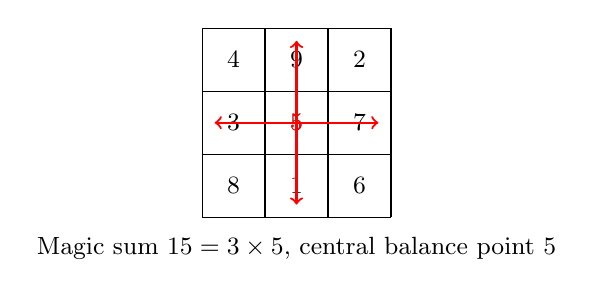
\begin{tikzpicture}[scale=0.8, every node/.style={font=\small}]
  \draw (0,0) grid (3,3);
  \node at (0.5,2.5) {4}; \node at (1.5,2.5) {9}; \node at (2.5,2.5) {2};
  \node at (0.5,1.5) {3}; \node at (1.5,1.5) {5}; \node at (2.5,1.5) {7};
  \node at (0.5,0.5) {8}; \node at (1.5,0.5) {1}; \node at (2.5,0.5) {6};
  \node[red] at (1.5,1.5) {5};
  \draw[->, thick, red] (1.5,1.5) -- (1.5,2.8);
  \draw[->, thick, red] (1.5,1.5) -- (1.5,0.2);
  \draw[->, thick, red] (1.5,1.5) -- (0.2,1.5);
  \draw[->, thick, red] (1.5,1.5) -- (2.8,1.5);
  \node at (1.5,-0.5) {Magic sum $15=3\times 5$, central balance point $5$};
\end{tikzpicture}
\caption{The Lo Shu matrix: a $3\times 3$ magic square with centre $5$ as the balance point and magic sum $15=3\times 5$.}
\label{fig:luoshu_matrix}
\end{figure}

\begin{definition}[Row Sums, Column Sums, and Diagonal Sums]\label{def:luoshu_line_sums}
For a $3 \times 3$ matrix $\mathbf{L} = (L_{ij})$, define:
\begin{enumerate}[label=(\roman*)]
    \item the \textbf{row sums} $r_i := \sum_{j=1}^{3} L_{ij}$ ($i = 1, 2, 3$);
    \item the \textbf{column sums} $c_j := \sum_{i=1}^{3} L_{ij}$ ($j = 1, 2, 3$);
    \item the \textbf{main diagonal sum} $d_+ := L_{11} + L_{22} + L_{33}$;
    \item the \textbf{anti-diagonal sum} $d_- := L_{13} + L_{22} + L_{31}$.
\end{enumerate}
\end{definition}

\begin{proposition}[Magic Square Property of the Lo Shu Matrix]\label{prop:luoshu_magic_sum}
The Lo Shu matrix $\mathbf{L}$ satisfies: all row sums, column sums, the main diagonal sum and the anti-diagonal sum are equal to $15$, that is,
\[
r_1 = r_2 = r_3 = c_1 = c_2 = c_3 = d_+ = d_- = 15 = 3 \times 5.
\]
$\mathbf{L}$ is called a \textbf{magic square of order three}, and $15$ is called its \textbf{magic sum}.
\end{proposition}

\begin{proof}
Direct computation:
\begin{align*}
r_1 &= 4 + 9 + 2 = 15, \quad r_2 = 3 + 5 + 7 = 15, \quad r_3 = 8 + 1 + 6 = 15; \\
c_1 &= 4 + 3 + 8 = 15, \quad c_2 = 9 + 5 + 1 = 15, \quad c_3 = 2 + 7 + 6 = 15; \\
d_+ &= 4 + 5 + 6 = 15, \quad d_- = 2 + 5 + 8 = 15.
\end{align*}
The sums of all eight lines are $15 = 3 \times 5$.
\end{proof}

\begin{definition}[Lo Shu Balance Point]\label{def:luoshu_balance_point}
The central entry $L_{22} = 5$ of $\mathbf{L}$ is called the \textbf{Lo Shu balance point}.
\end{definition}

\begin{proposition}[Triple Characterisation of the Balance Point]\label{prop:luoshu_balance_triple}
The Lo Shu balance point $5$ satisfies the following three equivalent characterisations:
\begin{enumerate}[label=(\roman*)]
    \item \textbf{Arithmetic centre}: $5 = \dfrac{1 + 2 + \cdots + 9}{9}$, that is, $5$ is the arithmetic mean of $1$ to $9$;
    \item \textbf{Magic sum factor}: $15 = 3 \times 5$, so the magic sum is exactly three times the balance point;
    \item \textbf{Diagonal mean}: the means of the two diagonals are both $5$, that is, $\dfrac{d_+}{3} = \dfrac{d_-}{3} = 5$.
\end{enumerate}
\end{proposition}

\begin{proof}
(i) $\dfrac{1 + 2 + \cdots + 9}{9} = \dfrac{45}{9} = 5$.
(ii) By Proposition \ref{prop:luoshu_magic_sum}, the magic sum is $15 = 3 \times 5$.
(iii) Dividing $d_+ = d_- = 15$ by $3$ gives $5$.
\end{proof}

\begin{proposition}[Lo Shu Antipodal Balancing]\label{prop:luoshu_antipodal}
The sums of the entries at antipodal positions of the Lo Shu matrix about the centre $5$ are always $10 = 2 \times 5$:
\[
L_{11} + L_{33} = 10, \quad L_{22} + L_{22} = 10, \quad L_{33} + L_{11} = 10,
\]
\[
L_{12} + L_{32} = 10, \quad L_{21} + L_{23} = 10, \quad L_{13} + L_{31} = 10.
\]
Equivalently, $\mathbf{L} - 5\mathbf{J}$ (where $\mathbf{J}$ is the all-ones matrix) satisfies the antipodal antisymmetry condition:
\[
(\mathbf{L} - 5\mathbf{J})_{ij} = -(\mathbf{L} - 5\mathbf{J})_{4-i, 4-j}, \quad i, j \in \{1, 2, 3\}.
\]
\end{proposition}

\begin{proof}
Direct computation of all antipodal pairs:
\[
4 + 6 = 10, \quad 9 + 1 = 10, \quad 2 + 8 = 10, \quad 3 + 7 = 10, \quad 5 + 5 = 10.
\]
For the second identity, note that $(\mathbf{L} - 5\mathbf{J})_{11} = 4 - 5 = -1$ and $(\mathbf{L} - 5\mathbf{J})_{33} = 6 - 5 = 1$, which are negatives of one another; the remaining antipodal positions are analogous.
\end{proof}

\begin{theorem}[Eigenvalues and Spectral Structure of the Lo Shu Matrix]\label{thm:luoshu_eigenvalues}
The characteristic polynomial of the Lo Shu matrix $\mathbf{L}$ is
\[
p(\lambda) = \det(\mathbf{L} - \lambda \mathbf{I}) = -(\lambda - 15)(\lambda^2 + 24).
\]
Hence the three eigenvalues of $\mathbf{L}$ are
\[
\lambda_1 = 15, \qquad \lambda_{2,3} = \pm 2\sqrt{6}\, i.
\]
The eigenvalue $\lambda_1 = 15 = 3 \times 5$ is a positive real eigenvalue, corresponding to pure translation; $\lambda_{2,3} = \pm 2\sqrt{6} i$ are a purely imaginary conjugate pair, of modulus $|\lambda_{2,3}| = 2\sqrt{6}$, corresponding to the joint action of rotation and scaling in the two-dimensional real invariant subspace.
\end{theorem}

\begin{proof}
Compute the characteristic polynomial:
\begin{align*}
p(\lambda) &= \det \begin{pmatrix} 4 - \lambda & 9 & 2 \\ 3 & 5 - \lambda & 7 \\ 8 & 1 & 6 - \lambda \end{pmatrix} \\
&= (4 - \lambda)\bigl[(5-\lambda)(6-\lambda) - 7\bigr] - 9\bigl[3(6-\lambda) - 56\bigr] + 2\bigl[3 - 8(5-\lambda)\bigr] \\
&= (4-\lambda)(\lambda^2 - 11\lambda + 23) + 9(38 + 3\lambda) - 2(37 - 8\lambda) \\
&= -\lambda^3 + 15\lambda^2 - 24\lambda + 360 \\
&= -(\lambda - 15)(\lambda^2 + 24).
\end{align*}
Solving $p(\lambda) = 0$ gives $\lambda_1 = 15$ and $\lambda_{2,3}^2 = -24$, that is, $\lambda_{2,3} = \pm 2\sqrt{6}\, i$.
\end{proof}

\begin{theorem}[Translation-Rotation Decomposition of the Lo Shu Matrix]\label{thm:luoshu_decomposition}
The Lo Shu matrix $\mathbf{L}$ decomposes into the sum of a pure translation part and a rotation-and-scaling part:
\[
\mathbf{L} = \underbrace{5\mathbf{J}}_{\text{translation part}} + \underbrace{(\mathbf{L} - 5\mathbf{J})}_{\text{rotation-and-scaling part}},
\]
where $\mathbf{J}$ is the all-ones matrix. These two parts satisfy:
\begin{enumerate}[label=(\roman*)]
    \item \textbf{Translation part} $5\mathbf{J}$: it acts on the vector $\mathbf{1} = (1,1,1)^{\mathsf T}$ as $15\mathbf{1}$, whilst it acts as zero on $\mathbf{1}^\perp$; that is, the eigenvalues of $5\mathbf{J}$ are $15, 0, 0$.
    \item \textbf{Rotation-and-scaling part} $\mathbf{L} - 5\mathbf{J}$: it acts as zero on $\mathbf{1}$, whilst on $\mathbf{1}^\perp$ it has eigenvalues $\pm 2\sqrt{6}i$ (of modulus $2\sqrt{6}\ne1$).
\end{enumerate}
Consequently $\mathbf{L}$ is a pure translation on the invariant subspace $\operatorname{span}(\mathbf{1})$ and acts on the invariant subspace $\mathbf{1}^\perp$ as a joint rotation and scaling: rotation through $\pi/2$ combined with scaling of the modulus by $2\sqrt{6}$ at each step (this is not a pure rotation, since a pure rotation requires $|\lambda|=1$ whilst here $|\lambda_{2,3}|=2\sqrt{6}\ne1$).
\end{theorem}

\begin{proof}
\textbf{Translation part}: $5\mathbf{J}$ maps any vector $\mathbf{v}$ to $5(\mathbf{1}^{\mathsf T}\mathbf{v})\mathbf{1}$. Hence $5\mathbf{J}\mathbf{1} = 5 \cdot 3\mathbf{1} = 15\mathbf{1}$, and for $\mathbf{v} \in \mathbf{1}^\perp$ (that is, $\mathbf{1}^{\mathsf T}\mathbf{v} = 0$) we have $5\mathbf{J}\mathbf{v} = \mathbf{0}$.

\textbf{Rotation-and-scaling part}: by Proposition \ref{prop:luoshu_magic_sum}, every row sum is $15$, so $(\mathbf{L} - 5\mathbf{J})\mathbf{1} = \mathbf{L}\mathbf{1} - 5\mathbf{J}\mathbf{1} = 15\mathbf{1} - 15\mathbf{1} = \mathbf{0}$. Hence $\mathbf{1}$ lies in the null space.

\textbf{Consistency of the eigenvalues}: let $\mathbf{v} \in \mathbf{1}^\perp$ be an eigenvector of $\mathbf{L} - 5\mathbf{J}$ with eigenvalue $\mu$. Then $\mathbf{L}\mathbf{v} = (5\mathbf{J} + (\mathbf{L} - 5\mathbf{J}))\mathbf{v} = \mathbf{0} + \mu\mathbf{v} = \mu\mathbf{v}$. Hence $\mathbf{v}$ is also an eigenvector of $\mathbf{L}$ with eigenvalue $\mu$. By Theorem \ref{thm:luoshu_eigenvalues}, the eigenvalues of $\mathbf{L}$ on $\mathbf{1}^\perp$ are $\pm 2\sqrt{6}i$. A direct computation of $\det(\mathbf{L} - 5\mathbf{J} - \lambda I)$ likewise verifies $-\lambda(\lambda^2 + 24)$.
\end{proof}

\begin{corollary}[Structural Significance of the Lo Shu Balance Point and Magic Sum]\label{cor:luoshu_grammar}
The spectral structure of the Lo Shu matrix reveals the twofold significance of the balance point $5$ and the magic sum $15$ at the level of the two operators:
\begin{enumerate}[label=(\roman*)]
    \item \textbf{On the gradient side}: $5 = 15/3$ is the average scale of the pure translation along the all-ones direction---the stretching factor of the translation part $5\mathbf{J}$ in the $\mathbf{1}$ direction is $15$, and dividing by the dimension $3$ gives the average factor $5$ per component;
    \item \textbf{On the curl side}: $5$ is the centre of the antipodal balance---the antipodal antisymmetry of $\mathbf{L} - 5\mathbf{J}$ (Proposition \ref{prop:luoshu_antipodal}) has $5$ as its axis of symmetry;
    \item \textbf{On the period side}: $\mathbf{L}$ has the rotation-and-scaling eigenvalues $\pm 2\sqrt{6}i$ on $\mathbf{1}^\perp$, corresponding to rotation through $\pi/2$ and scaling of the modulus by $2\sqrt{6}$ at each step in that two-dimensional real invariant subspace; since $|\lambda_{2,3}|=2\sqrt{6}\ne1$, the orbit does not close.
\end{enumerate}
\end{corollary}

\begin{proof}
(i) By Theorem \ref{thm:luoshu_decomposition}, $5\mathbf{J}$ has the eigenvalue $15$ in the $\mathbf{1}$ direction; its mean is $15/3 = 5$. (ii) By Proposition \ref{prop:luoshu_antipodal}, $\mathbf{L} - 5\mathbf{J}$ is antipodally antisymmetric about $5$. (iii) By Theorem \ref{thm:luoshu_eigenvalues} and $\lambda_{2,3} = \pm 2\sqrt{6}i$, a purely imaginary eigenvalue $\pm2\sqrt{6}i$ has modulus $2\sqrt{6}\ne1$, corresponding to rotation through $\pi/2$ and scaling of the modulus by $2\sqrt{6}$ at each step, so the orbit does not close.
\end{proof}

\begin{example}[Spectral Decomposition of the Lo Shu Matrix]\label{ex:luoshu_spectral}
The eigenvectors corresponding to the three eigenvalues of the Lo Shu matrix $\mathbf{L}$ are as follows:
\begin{enumerate}[label=(\roman*)]
    \item $\lambda_1 = 15$: the eigenvector $\mathbf{v}_1 = \frac{1}{\sqrt{3}}(1,1,1)^{\mathsf T}$ (all components equal);
    \item $\lambda_2 = 2\sqrt{6}i$ and $\lambda_3 = -2\sqrt{6}i$: the eigenvectors lie inside $\mathbf{1}^\perp$.
\end{enumerate}
Verification for $\mathbf{v}_1$: $\mathbf{L}\mathbf{v}_1 = \frac{1}{\sqrt{3}}(15, 15, 15)^{\mathsf T} = 15\mathbf{v}_1$.

Take an orthonormal basis of $\mathbf{1}^\perp$ to be $\mathbf{e}_2 = \frac{1}{\sqrt{2}}(1, -1, 0)^{\mathsf T}$ and $\mathbf{e}_3 = \frac{1}{\sqrt{6}}(1, 1, -2)^{\mathsf T}$; the matrix of the restriction $\mathbf{L}|_{\mathbf{1}^\perp}$ of $\mathbf{L}$ to $\mathbf{1}^\perp$ with respect to this basis is
\[
\mathbf{L}|_{\mathbf{1}^\perp} = \begin{pmatrix} -\frac{3}{2} & \frac{5\sqrt{3}}{2} \\ -\frac{7\sqrt{3}}{2} & \frac{3}{2} \end{pmatrix}
\]
Its characteristic polynomial is $\mu^2 + 24$, whose roots are $\mu = \pm 2\sqrt{6}\,i$, in agreement with the non-zero roots of the complete characteristic polynomial $-\lambda(\lambda^2 + 24)$ (the action of $\mathbf{L}$ on $\mathbf{1}^\perp$ is equivalent to a rotation through $\pi/2$ combined with a scaling of the modulus by $2\sqrt{6}$).
\end{example}

\begin{remark}[Lo Shu Matrix and the Interface with $\mathbb{Z}_2 \times \mathbb{Z}_5$ Structure]\label{rem:luoshu_hetu_interface}
The factor $5$ in the magic sum $15 = 3 \times 5$ of the Lo Shu matrix is algebraically related to the $\mathbb{Z}_5$ component of $\mathbb{Z}_{10} \cong \mathbb{Z}_2 \times \mathbb{Z}_5$ in Chapter 6: the Lo Shu centre $5$ corresponds to the reference point of the $\mathbb{Z}_5$ component, whilst the antipodal balance of the Lo Shu matrix (with sum $10 = 2 \times 5$) corresponds to the double alternation of $\mathbb{Z}_2$. The complex conjugate eigenvalues $\pm 2\sqrt{6}i$ of the Lo Shu matrix on $\mathbf{1}^\perp$ provide a concrete example: every step in that two-dimensional real invariant subspace is a rotation through $\pi/2$ combined with a scaling of the modulus by $2\sqrt{6}$, and both the angle and the scaling factor are entirely determined by the algebraic structure of the matrix.
\end{remark}


\section{\texorpdfstring{Lie Groups: a Rigorous Formulation of Continuous Symmetry Groups}{Lie Groups}}

\begin{definition}[Lie Group]\label{def:lie_group}
A \textbf{Lie group} is a smooth manifold $G$ equipped with a group structure $(G, \cdot)$ such that the group operations
\[
\mu: G \times G \to G, \quad (g, h) \mapsto g \cdot h, \quad
\iota: G \to G, \quad g \mapsto g^{-1}
\]
are both smooth maps.

A Lie group unifies the abstract concept of a group in the `Operations and Periodicity' chapter with the concept of a smooth manifold. The three basic transformation groups of periodic mathematics---the translation group, the scaling group and the rotation group---are all Lie groups.
\end{definition}

\begin{example}[The three transformation groups are Lie groups]\label{ex:three_lie_groups}
\begin{enumerate}[label=(\roman*)]
    \item \textbf{Translation group} $(\mathbb{R}^n, +)$: as a manifold it is $\mathbb{R}^n$, the group operation is vector addition, and it is smooth. An Abelian Lie group.
    \item \textbf{Scaling group} $(\mathbb{R}^+, \times)$: as a manifold it is the positive real axis $(0, \infty)$, the group operation is multiplication, and it is smooth. An Abelian Lie group, isomorphic as a Lie group to $(\mathbb{R}, +)$ via the exponential map $\exp$.
    \item \textbf{Rotation group} $U(1) = \{z \in \mathbb{C} : |z| = 1\}$: as a manifold it is the circle $S^1$, the group operation is complex multiplication, and it is smooth. A compact, connected, Abelian Lie group.
\end{enumerate}
\end{example}

\begin{figure}[htbp]
\centering
\begin{tikzpicture}[
  box/.style={draw, rounded corners, align=center, inner sep=5pt, font=\small},
  arr/.style={->, thick, >=stealth}
]
  \node[box, fill=blue!8] (trans) {Translation group\\$(\mathbb R^n,+)$};
  \node[box, fill=orange!12, right=1.2cm of trans] (scale) {Scaling group\\$(\mathbb R^+,\times)$};
  \node[box, fill=green!12, right=1.2cm of scale] (rot) {Rotation group\\$U(1)=S^1$};
  \node[box, fill=red!8, below=1.0cm of trans] (exp1) {$\exp(X)=X$};
  \node[box, fill=purple!8, below=1.0cm of scale] (exp2) {$\exp(s)=e^s$};
  \node[box, fill=cyan!8, below=1.0cm of rot] (exp3) {$\exp(i\theta)=e^{i\theta}$};
  \draw[arr] (trans) -- (exp1);
  \draw[arr] (scale) -- (exp2);
  \draw[arr] (rot) -- (exp3);
\end{tikzpicture}
\caption{The three transformation Lie groups and their exponential maps: the exponential of the translation group is the identity, that of the scaling group is the real exponential, and that of the rotation group is the complex exponential.}
\label{fig:lie_groups}
\end{figure}

\begin{proposition}[One-parameter Subgroup]\label{prop:one_parameter_subgroup}
Let $G$ be a Lie group and let $X \in T_eG$ be a tangent vector at the identity element $e$. Then there exists a unique Lie group homomorphism $\gamma_X: \mathbb{R} \to G$ satisfying $\dot{\gamma}_X(0) = X$. The map $\gamma_X$ is called the \textbf{one-parameter subgroup} generated by $X$. It satisfies
\[
\gamma_X(s + t) = \gamma_X(s) \cdot \gamma_X(t), \qquad \forall s, t \in \mathbb{R}.
\]
\end{proposition}

\begin{proof}
This is a fundamental theorem of Lie group theory. Existence is guaranteed by the existence and uniqueness theorem for ordinary differential equations: $\gamma_X$ is the integral curve of the left-invariant vector field $X^L$ ($X^L(g) = dL_g(X)$). Uniqueness and the homomorphism property follow from the properties of the flow of a left-invariant vector field: if $\gamma_X$ is the integral curve of $X^L$ satisfying $\gamma_X(0) = e$, then both $t \mapsto \gamma_X(s+t)$ and $t \mapsto \gamma_X(s)\gamma_X(t)$ are integral curves of $X^L$ passing through $\gamma_X(s)$ at $t=0$, so by uniqueness they coincide.
\end{proof}

\begin{definition}[Exponential Map]\label{def:exponential_map}
Let $G$ be a Lie group. The \textbf{exponential map} $\exp: T_eG \to G$ is defined by $\exp(X) := \gamma_X(1)$, where $\gamma_X$ is the one-parameter subgroup generated by $X$. The exponential map sends a tangent vector at the identity (an infinitesimal transformation) to a group element (a finite transformation).
\end{definition}

\begin{proposition}[Exponential maps of the three transformation groups]\label{prop:three_exponential_maps}
\begin{enumerate}[label=(\roman*)]
    \item \textbf{Translation group} $(\mathbb{R}^n, +)$: $T_eG \cong \mathbb{R}^n$, $\exp(X) = X$. The one-parameter subgroup is $\gamma_X(t) = tX$.
    \item \textbf{Scaling group} $(\mathbb{R}^+, \times)$: $T_eG \cong \mathbb{R}$, $\exp(s) = e^s$. The one-parameter subgroup is $\gamma_s(t) = e^{st}$.
    \item \textbf{Rotation group} $U(1)$: $T_eG \cong i\mathbb{R} \cong \mathbb{R}$, $\exp(i\theta) = e^{i\theta}$. The one-parameter subgroup is $\gamma_{i\theta}(t) = e^{i\theta t}$.
\end{enumerate}
\end{proposition}

\begin{proof}
(i) On the translation group the left-invariant vector field is the constant vector field $X^L(g) = X$. Its integral curve satisfies $\dot{\gamma}(t) = X$ and $\gamma(0) = 0$, giving $\gamma(t) = tX$. Hence $\exp(X) = \gamma_X(1) = X$.

(ii) On the scaling group, the tangent vector $s \in \mathbb{R}$ at the identity $e = 1$ corresponds to the left-invariant vector field $X^L(x) = sx$. The integral curve satisfies $\dot{\gamma}(t) = s\gamma(t)$ and $\gamma(0) = 1$, giving $\gamma(t) = e^{st}$. Hence $\exp(s) = e^s$.

(iii) On the rotation group, the tangent vector $i\theta$ at the identity $e = 1$ corresponds to the left-invariant vector field $X^L(z) = i\theta z$. The integral curve satisfies $\dot{\gamma}(t) = i\theta\gamma(t)$ and $\gamma(0) = 1$, giving $\gamma(t) = e^{i\theta t}$. Hence $\exp(i\theta) = e^{i\theta}$.
\end{proof}

\begin{remark}[Correspondence between the Exponential Map and the Three Operators]\label{rem:exponential_grammar}
The exponential map is the bridge connecting \textbf{infinitesimal transformations} and \textbf{finite transformations}:
\begin{itemize}
    \item On the translation group $\exp = \text{id}$: an infinitesimal translation is a finite translation---the gradient (symmetry centre $0$) is `flat', and no exponentiation is needed.
    \item On the scaling group $\exp(s) = e^s$: the infinitesimal scaling $s$ becomes, through the exponential map, the finite scaling factor $e^s$---the divergence (symmetry centre $1$) accumulates by exponentiation.
    \item On the rotation group $\exp(i\theta) = e^{i\theta}$: the infinitesimal rotation angle $i\theta$ becomes, through the exponential map, the unit complex number $e^{i\theta}$---the curl (symmetry centre $i$) generates periodicity by exponentiation.
\end{itemize}
\end{remark}

\begin{proposition}[Finite-order Elements and Closed Orbits of a Lie Group]\label{prop:lie_group_finite_order}
Let $G$ be a Lie group and let $g = \exp(X) \in G$. If $g$ is an element of finite order ($\operatorname{ord}(g) = p < \infty$), then the one-parameter subgroup $\gamma_X$ is periodic, that is, there exists $T > 0$ such that $\gamma_X(T) = e$---take $T=p$ directly from $g^p=e$; in that case $\gamma_X$ defines a closed orbit of period $p$. The converse requires an additional arithmetic condition: let $\gamma_X$ be non-constant ($X\ne0$) with least positive period $T_0$; then $\gamma_X(T)=e$ if and only if $T/T_0\in\mathbb{Z}$, so, since $g=\gamma_X(1)$,
\[
\operatorname{ord}(g)<\infty \iff T_0 \text{ is a rational part of } 1,\text{ that is, } 1/T_0\in\mathbb{Q},
\]
and then $\operatorname{ord}(g)$ is the least element of $\{n\ge1: n/T_0\in\mathbb{Z}\}$. For example, take $G=U(1)\subset\mathbb{C}^\times$ and $X=2\pi i\sqrt2$; then $\gamma_X(T)=e^{2\pi i\sqrt2\,T}$ has least positive period $T_0=1/\sqrt2$, whilst $1/T_0=\sqrt2\notin\mathbb{Q}$, so $g=e^{2\pi i\sqrt2}$ has infinite order. Hence in general the periodicity of $\gamma_X$ is only a necessary condition for $g$ to have finite order.
\end{proposition}

\begin{proof}
Forward direction (the direction proved in the text: $g$ of finite order $\Rightarrow$ $\gamma_X$ periodic). If $\operatorname{ord}(g) = p$, then $g^p = e$, that is, $\gamma_X(1)^p = e$. By the homomorphism property, $\gamma_X(p) = \gamma_X(1)^p = e$, so $\gamma_X$ returns to the identity at $t = p$, and $\gamma_X$ is periodic, with period $p$.

The converse fails; its correct form is the displayed equivalence above. Write $A=\{T>0:\gamma_X(T)=e\}$. Since $\gamma_X$ is a homomorphism, $A$ is closed under addition and under taking integer multiples; when $X\ne0$ the curve $\gamma_X$ does not take the value $e$ near $t=0$ (its derivative at $t=0$ is non-zero), so $A$ is discrete in $\mathbb{R}_{>0}$ and has a least element $T_0$, with $A=T_0\mathbb{Z}_{>0}$. Hence $g^n=e=\gamma_X(n)$ if and only if $n\in T_0\mathbb{Z}_{>0}$, that is, $n/T_0\in\mathbb{Z}$; such a positive integer $n$ exists if and only if $1/T_0\in\mathbb{Q}$. For $T_0=1/\sqrt2$ (the case $G=U(1)$, $X=2\pi i\sqrt2$) we have $1/T_0=\sqrt2\notin\mathbb{Q}$, so $\operatorname{ord}(g)=\infty$ whilst $\gamma_X(1/\sqrt2)=e$. Thus `$g$ of finite order $\Rightarrow$ $\gamma_X$ periodic' holds; the converse holds only with the extra hypothesis $1/T_0\in\mathbb{Q}$, in which case the order of $g$ is the denominator of $1/T_0$.
\end{proof}

\section{\texorpdfstring{Lie Algebras: The Infinitesimal Structure of Matrix Groups}{Lie Algebras: The Infinitesimal Structure of Matrix Groups}}

\begin{definition}[Lie Algebra]\label{def:lie_algebra}
Let $\mathbb{F}$ be a field. A \textbf{Lie algebra} over $\mathbb{F}$ is a vector space $\mathfrak{g}$ equipped with a bilinear map $[\cdot, \cdot]: \mathfrak{g} \times \mathfrak{g} \to \mathfrak{g}$ (called the \textbf{Lie bracket}) satisfying:
\begin{enumerate}[label=(\roman*)]
    \item \textbf{Antisymmetry}: $[X, Y] = -[Y, X]$;
    \item \textbf{The Jacobi identity}: $[X, [Y, Z]] + [Y, [Z, X]] + [Z, [X, Y]] = 0$.
\end{enumerate}
\end{definition}

\begin{remark}[The Significance of Lie Algebras in Periodic Mathematics]\label{rem:lie_algebra_periodic_meaning}
A Lie algebra describes the \textbf{infinitesimal structure} of a continuous symmetry group. The elements of a Lie algebra are infinitesimal generators---they generate one-parameter subgroups, and one-parameter subgroups in turn generate closed orbits. The Lie bracket $[X,Y]$ measures the non-commutativity of two infinitesimal transformations---when $[X,Y] = 0$, the transformations generated by $X$ and $Y$ commute with one another; when $[X,Y] \neq 0$, they cannot commute.
\end{remark}

\begin{definition}[Matrix Lie Algebra]\label{def:matrix_lie_algebra}
Let $G \subseteq GL(n, \mathbb{F})$ be a matrix Lie group. The \textbf{Lie algebra} $\mathfrak{g}$ of $G$ is the tangent space of $G$ at the identity $I$:
\[
\mathfrak{g} := T_I G = \{\mathbf{X} \in M_n(\mathbb{F}) : e^{t\mathbf{X}} \in G, \; \forall t \in \mathbb{R}\},
\]
The Lie bracket is the matrix commutator $[\mathbf{X}, \mathbf{Y}] = \mathbf{XY} - \mathbf{YX}$.
\end{definition}

\begin{proposition}[Three Basic Matrix Lie Algebras]\label{prop:three_matrix_lie_algebras}
\begin{enumerate}[label=(\roman*)]
    \item \textbf{Orthogonal Lie algebra} $\mathfrak{o}(n) = \{\mathbf{X} \in M_n(\mathbb{R}) : \mathbf{X}^{\mathsf T} = -\mathbf{X}\}$;
    \item \textbf{Unitary Lie algebra} $\mathfrak{u}(n) = \{\mathbf{X} \in M_n(\mathbb{C}) : \mathbf{X}^* = -\mathbf{X}\}$;
    \item \textbf{Symplectic Lie algebra} $\mathfrak{sp}(2n) = \{\mathbf{X} : \mathbf{X}^{\mathsf T}\mathbf{J} + \mathbf{J}\mathbf{X} = \mathbf{0}\}$.
\end{enumerate}
\end{proposition}

\begin{proof}
(i) Let $\mathbf{X} \in \mathfrak{o}(n)$. Then $e^{t\mathbf{X}} \in O(n)$ for all $t$, that is, $(e^{t\mathbf{X}})^{\mathsf T} e^{t\mathbf{X}} = I$. Differentiating at $t = 0$ gives $\mathbf{X}^{\mathsf T} + \mathbf{X} = \mathbf{0}$, hence $\mathbf{X}^{\mathsf T} = -\mathbf{X}$. Conversely, if $\mathbf{X}$ is antisymmetric, then $(e^{t\mathbf{X}})^{\mathsf T} e^{t\mathbf{X}} = e^{-t\mathbf{X}} e^{t\mathbf{X}} = I$.

(ii) Let $\mathbf{X} \in \mathfrak{u}(n)$. Differentiating $(e^{t\mathbf{X}})^* e^{t\mathbf{X}} = I$ gives $\mathbf{X}^* + \mathbf{X} = \mathbf{0}$.

(iii) Let $\mathbf{X} \in \mathfrak{sp}(2n)$. Differentiating $(e^{t\mathbf{X}})^{\mathsf T} \mathbf{J} e^{t\mathbf{X}} = \mathbf{J}$ gives $\mathbf{X}^{\mathsf T}\mathbf{J} + \mathbf{J}\mathbf{X} = \mathbf{0}$.
\end{proof}

\begin{figure}[htbp]
\centering
\begin{tikzpicture}[
  box/.style={draw, rounded corners, align=center, inner sep=5pt, font=\small},
  arr/.style={->, thick, >=stealth}
]
  \node[box, fill=blue!8] (alg) {Lie algebra $\mathfrak g$\\tangent space $T_IG$};
  \node[box, fill=orange!12, right=1.2cm of alg] (bracket) {Lie bracket\\$[X,Y]=XY-YX$};
  \node[box, fill=green!12, right=1.2cm of bracket] (exp) {Exponential map\\$e^{tX}\in G$};
  \node[box, fill=red!8, below=1.0cm of exp] (group) {Lie group $G$\\continuous symmetry};
  \draw[arr] (alg) -- (bracket);
  \draw[arr] (bracket) -- (exp);
  \draw[arr] (exp) -- (group);
\end{tikzpicture}
\caption{From Lie algebra to Lie group: tangent space, Lie bracket and exponential map.}
\label{fig:lie_algebra}
\end{figure}

\begin{proposition}[Properties of the Matrix Exponential Map]\label{prop:matrix_exponential_properties}
Let $\mathbf{X} \in M_n(\mathbb{F})$. The matrix exponential $e^{\mathbf{X}}$ satisfies:
\begin{enumerate}[label=(\roman*)]
    \item $e^{\mathbf{0}} = \mathbf{I}$;
    \item $e^{\mathbf{X}} e^{-\mathbf{X}} = \mathbf{I}$;
    \item if $\mathbf{XY} = \mathbf{YX}$, then $e^{\mathbf{X}+\mathbf{Y}} = e^{\mathbf{X}} e^{\mathbf{Y}}$;
    \item $\det(e^{\mathbf{X}}) = e^{\operatorname{tr}(\mathbf{X})}$;
    \item if $\mathbf{X}$ is antisymmetric, then $e^{\mathbf{X}} \in SO(n)$;
    \item if $\mathbf{X}$ is skew-Hermitian, then $e^{\mathbf{X}} \in U(n)$.
\end{enumerate}
\end{proposition}

\begin{proof}
(i) Substitute directly into the power series definition.

(ii) Since $\mathbf{X}$ and $-\mathbf{X}$ commute, use (iii): $e^{\mathbf{X}} e^{-\mathbf{X}} = e^{\mathbf{X}-\mathbf{X}} = \mathbf{I}$.

(iii) When $\mathbf{XY} = \mathbf{YX}$, the binomial theorem gives $e^{\mathbf{X}} e^{\mathbf{Y}} = \sum_{m} \frac{(\mathbf{X}+\mathbf{Y})^m}{m!} = e^{\mathbf{X}+\mathbf{Y}}$.

(iv) Let the eigenvalues of the Jordan normal form of $\mathbf{X}$ be $\lambda_1, \dots, \lambda_n$. Then the eigenvalues of $e^{\mathbf{X}}$ are $e^{\lambda_1}, \dots, e^{\lambda_n}$, hence $\det(e^{\mathbf{X}}) = e^{\sum_i \lambda_i} = e^{\operatorname{tr}(\mathbf{X})}$.

(v) By (i)--(iii), $e^{\mathbf{X}^{\mathsf T}} = (e^{\mathbf{X}})^{\mathsf T}$. If $\mathbf{X}^{\mathsf T} = -\mathbf{X}$, then $(e^{\mathbf{X}})^{\mathsf T} = e^{-\mathbf{X}} = (e^{\mathbf{X}})^{-1}$, so $e^{\mathbf{X}} \in O(n)$. By (iv), $\det(e^{\mathbf{X}}) = e^{\operatorname{tr}(\mathbf{X})} = 1$ (the trace of an antisymmetric matrix is zero), so $e^{\mathbf{X}} \in SO(n)$.

(vi) Similarly, $(e^{\mathbf{X}})^* = e^{-\mathbf{X}} = (e^{\mathbf{X}})^{-1}$, so $e^{\mathbf{X}} \in U(n)$.
\end{proof}

\begin{theorem}[Correspondence Between Lie Algebras and Conservation Laws]\label{thm:lie_algebra_conservation}
The elements of the three basic matrix Lie algebras generate matrix groups through the matrix exponential map, corresponding respectively to three conservation laws:
\begin{enumerate}[label=(\roman*)]
    \item \textbf{Orthogonal Lie algebra} $\mathfrak{o}(n)$: antisymmetric matrices generate $SO(n)$---preserving the real inner product ($0$-symmetry).
    \item \textbf{Unitary Lie algebra} $\mathfrak{u}(n)$: skew-Hermitian matrices generate $U(n)$---preserving the complex inner product (conservation of angular momentum, curl operator, $i$-symmetry).
    \item \textbf{Symplectic Lie algebra} $\mathfrak{sp}(2n)$: generates $Sp(2n)$---preserving the symplectic form (conservation of phase-space volume, divergence operator, $1$-symmetry).
\end{enumerate}
\end{theorem}

\begin{proof}
This follows directly from Proposition \ref{prop:three_matrix_lie_algebras} and parts (v)(vi) of Proposition \ref{prop:matrix_exponential_properties}: the exponential map of $\mathfrak{o}(n)$ lands in $SO(n)$, that of $\mathfrak{u}(n)$ lands in $U(n)$, and that of $\mathfrak{sp}(2n)$ lands in $Sp(2n)$.
\end{proof}

\begin{example}[$\mathfrak{su}(2)$ and Three-Dimensional Rotation]\label{ex:su2_rotation}
The Lie algebra of the three-dimensional rotation group $SO(3)$ is $\mathfrak{so}(3)$, consisting of the $3 \times 3$ antisymmetric matrices:
\[
\mathfrak{so}(3) = \operatorname{span}\left\{
\begin{pmatrix} 0 & 0 & 0 \\ 0 & 0 & -1 \\ 0 & 1 & 0 \end{pmatrix},
\begin{pmatrix} 0 & 0 & 1 \\ 0 & 0 & 0 \\ -1 & 0 & 0 \end{pmatrix},
\begin{pmatrix} 0 & -1 & 0 \\ 1 & 0 & 0 \\ 0 & 0 & 0 \end{pmatrix}
\right\}.
\]
The three generators $J_x, J_y, J_z$ satisfy the angular momentum commutation relations $[J_x, J_y] = J_z$, $[J_y, J_z] = J_x$, $[J_z, J_x] = J_y$. The exponential map $e^{\theta J_z}$ gives the rotation matrix through the angle $\theta$ about the $z$ axis. The Lie algebra $\mathfrak{su}(2)$ is isomorphic to $\mathfrak{so}(3)$, and is the expression at the level of Lie algebras of the double cover $SU(2) \to SO(3)$.
\end{example}


\section{\texorpdfstring{Singular Value Decomposition and Periodic Convolution}{Singular Value Decomposition and Periodic Convolution}}

\begin{definition}[Singular Value Decomposition]\label{def:svd}
Let $\mathbf{A}$ be an $m \times n$ complex matrix. The \textbf{singular value decomposition} (SVD) of $\mathbf{A}$ is
\[
\mathbf{A} = \mathbf{U} \boldsymbol{\Sigma} \mathbf{V}^*,
\]
where $\mathbf{U}$ is an $m \times m$ unitary matrix, $\mathbf{V}$ is an $n \times n$ unitary matrix, and $\boldsymbol{\Sigma}$ is an $m \times n$ diagonal matrix whose diagonal entries $\sigma_1 \ge \sigma_2 \ge \dots \ge \sigma_r > 0$ are the \textbf{singular values} of $\mathbf{A}$ ($r = \operatorname{rank}(\mathbf{A})$).

The singular value decomposition is the matrix realisation of periodic convolution: the columns of $\mathbf{U}$ are the rotation axes of the output space, the columns of $\mathbf{V}$ are the rotation axes of the input space, and the diagonal entries of $\boldsymbol{\Sigma}$ are the scaling factors of the corresponding channels.
\end{definition}

\begin{figure}[htbp]
\centering
\begin{tikzpicture}[
  box/.style={draw, rounded corners, align=center, inner sep=5pt, font=\small},
  arr/.style={->, thick, >=stealth}
]
  \node[box, fill=blue!8] (in) {Input space};
  \node[box, fill=orange!12, right=1.0cm of in] (V) {$\mathbf V^*$\\rotation};
  \node[box, fill=green!12, right=1.0cm of V] (S) {$\boldsymbol\Sigma$\\scaling};
  \node[box, fill=red!8, right=1.0cm of S] (U) {$\mathbf U$\\rotation};
  \node[box, fill=purple!8, right=1.0cm of U] (out) {Output space};
  \draw[arr] (in) -- (V);
  \draw[arr] (V) -- (S);
  \draw[arr] (S) -- (U);
  \draw[arr] (U) -- (out);
\end{tikzpicture}
\caption{The geometric meaning of the singular value decomposition: rotation-scaling-rotation.}
\label{fig:svd_geometry}
\end{figure}

\begin{proposition}[SVD and the Correspondence with the Four Operators of Periodic Convolution]\label{prop:svd_periodic_transform}
The geometric meaning of the singular value decomposition corresponds precisely to the four-operator structure of periodic convolution:
\begin{enumerate}[label=(\roman*)]
    \item \textbf{Phase operator} (rotation) $\leftrightarrow$ $\mathbf{V}^*$ and $\mathbf{U}$: the rotation axes of the input/output space;
    \item \textbf{Amplitude operator} (scaling) $\leftrightarrow$ $\boldsymbol{\Sigma}$: each channel is scaled independently by the singular value $\sigma_i$;
    \item \textbf{Frequency operator} (translation) $\leftrightarrow$ the DFT diagonalisation of a circulant matrix: when $\mathbf{A}$ is a circulant matrix, $\mathbf{U} = \mathbf{F}_N^* \operatorname{diag}(e^{i\phi_k})$, $\mathbf{V} = \mathbf{F}_N^*$ and $\boldsymbol{\Sigma} = \operatorname{diag}(|\hat{a}_0|, \dots, |\hat{a}_{N-1}|)$, where $\hat{a}_k = |\hat{a}_k| e^{i\phi_k}$;
    \item \textbf{Period operator} (fixed length) $\leftrightarrow$ block circulant structure: nested periodic systems correspond to block circulant matrices, whose SVD is carried out in layers according to the period class.
\end{enumerate}
\end{proposition}

\begin{proof}
(i)(ii) These are read off directly from the definition of the singular value decomposition (Definition \ref{def:svd}): the action of $\mathbf{A} = \mathbf{U}\boldsymbol{\Sigma}\mathbf{V}^*$ first performs the rotation $\mathbf{V}^*$ in the input space, then scales each channel independently by the corresponding singular value $\sigma_i$, and finally performs the rotation $\mathbf{U}$ in the output space.

(iii) Let $\mathbf{A}$ be the circulant matrix with first row $\mathbf{a} = (a_0, a_1, \dots, a_{N-1})$; its $j$-th column is obtained by cyclically shifting $\mathbf{a}$, so $\mathbf{A}$ commutes with the cyclic shift operator and is therefore unitarily diagonalised by the DFT matrix $\mathbf{F}_N$:
\[
\mathbf{A} = \mathbf{F}_N^* \operatorname{diag}(\hat{a}_0, \hat{a}_1, \dots, \hat{a}_{N-1})\, \mathbf{F}_N, \qquad \hat{a}_k = \sum_{j=0}^{N-1} a_j e^{-2\pi i jk/N}.
\]
Writing each $\hat{a}_k = |\hat{a}_k| e^{i\phi_k}$ in terms of modulus and phase gives
\[
\mathbf{A} = \bigl(\mathbf{F}_N^* \operatorname{diag}(e^{i\phi_k})\bigr)\, \operatorname{diag}(|\hat{a}_0|, \dots, |\hat{a}_{N-1}|)\, \mathbf{F}_N,
\]
which is precisely the SVD form of $\mathbf{A}$.

(iv) Nested periodic systems correspond to block circulant matrices, whose DFT diagonalisation generalises to a block DFT, and the singular values are given in layers according to the period class.
\end{proof}

\begin{proposition}[Singular Values and Conserved Quantities]\label{prop:svd_conservation}
The singular values of a matrix $\mathbf{A}$ satisfy the following conservation properties:
\begin{enumerate}[label=(\roman*)]
    \item \textbf{Conservation of the Frobenius norm}: $\|\mathbf{A}\|_F^2 = \sum_{i=1}^r \sigma_i^2$---the `total energy' of the matrix equals the sum of the squares of its singular values; this is the matrix version of Parseval's identity.
    \item \textbf{Conservation of rank}: $\operatorname{rank}(\mathbf{A}) = r$, equal to the number of non-zero singular values.
    \item \textbf{Conservation of the determinant} (square case): $|\det(\mathbf{A})| = \prod_{i=1}^n \sigma_i$.
\end{enumerate}
\end{proposition}

\begin{proof}
(i) From $\mathbf{A} = \mathbf{U}\boldsymbol{\Sigma}\mathbf{V}^*$ and unitary invariance, $\|\mathbf{A}\|_F^2 = \operatorname{tr}(\mathbf{A}^*\mathbf{A}) = \operatorname{tr}(\mathbf{V}\boldsymbol{\Sigma}^*\boldsymbol{\Sigma}\mathbf{V}^*) = \operatorname{tr}(\boldsymbol{\Sigma}^*\boldsymbol{\Sigma}) = \sum_{i=1}^r \sigma_i^2$.

(ii) Since $\mathbf{U}, \mathbf{V}$ are invertible, $\operatorname{rank}(\mathbf{A}) = \operatorname{rank}(\boldsymbol{\Sigma})$, and the rank of $\boldsymbol{\Sigma}$ is precisely the number $r$ of its non-zero diagonal entries.

(iii) In the square case, taking determinants gives $\det(\mathbf{A}) = \det(\mathbf{U})\det(\boldsymbol{\Sigma})\det(\mathbf{V}^*)$; since $\mathbf{U}, \mathbf{V}$ are unitary matrices, $|\det(\mathbf{U})| = |\det(\mathbf{V}^*)| = 1$, hence $|\det(\mathbf{A})| = |\det(\boldsymbol{\Sigma})| = \prod_{i=1}^n \sigma_i$.
\end{proof}

\begin{example}[Singular Value Decomposition of a $2\times 2$ Matrix]\label{ch5_example_svd_2x2}
Consider the matrix $\mathbf{A} = \begin{pmatrix} 0 & 3 \\ 4 & 0 \end{pmatrix}$. A computation gives $\mathbf{A}^{\mathsf T}\mathbf{A} = \begin{pmatrix} 16 & 0 \\ 0 & 9 \end{pmatrix}$, whose eigenvalues are $16, 9$, so the singular values are $\sigma_1 = 4 \ge \sigma_2 = 3$. Take
\[
\mathbf{U} = \begin{pmatrix} 0 & 1 \\ 1 & 0 \end{pmatrix}, \qquad \boldsymbol{\Sigma} = \begin{pmatrix} 4 & 0 \\ 0 & 3 \end{pmatrix}, \qquad \mathbf{V} = \mathbf{I}_2,
\]
so that $\mathbf{U}\boldsymbol{\Sigma}\mathbf{V}^{\mathsf T} = \mathbf{A}$. Verifying the conserved quantities: $|\det\mathbf{A}| = 12 = \sigma_1\sigma_2$ and $\|\mathbf{A}\|_F^2 = 25 = \sigma_1^2 + \sigma_2^2$.
\end{example}

\begin{definition}[Pseudoinverse and Least Squares]\label{def:pseudoinverse}
Let $\mathbf{A} = \mathbf{U} \boldsymbol{\Sigma} \mathbf{V}^*$ be an SVD. The \textbf{Moore-Penrose pseudoinverse} of $\mathbf{A}$ is $\mathbf{A}^+ = \mathbf{V} \boldsymbol{\Sigma}^+ \mathbf{U}^*$, where $\boldsymbol{\Sigma}^+$ is the diagonal matrix with diagonal entries $1/\sigma_i$ ($\sigma_i > 0$) or $0$ ($\sigma_i = 0$). The pseudoinverse gives the least squares solution of an inconsistent system of linear equations $\mathbf{A}\mathbf{x} = \mathbf{b}$: $\mathbf{x} = \mathbf{A}^+ \mathbf{b}$ minimises $\|\mathbf{A}\mathbf{x} - \mathbf{b}\|^2$.
\end{definition}

\section{\texorpdfstring{The Periodic Structure of Linear Systems}{The Periodic Structure of Linear Systems}}

\begin{definition}[Linear Dynamical System]\label{def:linear_dynamical_system}
A \textbf{discrete linear dynamical system} has the form $\mathbf{x}_{k+1} = \mathbf{A} \mathbf{x}_k$. A \textbf{continuous linear dynamical system} has the form $\frac{d\mathbf{x}}{dt} = \mathbf{B} \mathbf{x}$. These two systems are related through the matrix exponential: the solution of the continuous system is $\mathbf{x}(t) = e^{\mathbf{B}t} \mathbf{x}(0)$, which, after discretisation with time step $\Delta t$, corresponds to $\mathbf{A} = e^{\mathbf{B}\Delta t}$.
\end{definition}

\begin{proposition}[Periodic Solutions of Linear Systems]\label{prop:linear_system_periodic_solution}
Let the eigenvalues of $\mathbf{A}$ be $\lambda_1, \dots, \lambda_n$. The discrete system $\mathbf{x}_{k+1} = \mathbf{A} \mathbf{x}_k$ has a periodic solution of period $p$ (that is, $\mathbf{x}_{k+p} = \mathbf{x}_k$ for all $k$) if and only if there exists an eigenvalue $\lambda_j$ satisfying $\lambda_j^p = 1$ and the initial value lies in the direct sum $\bigoplus_{\lambda_j^p=1}E_{\lambda_j}$ of the eigenspaces of those eigenvalues. No diagonalisability of $\mathbf{A}$ is needed here: what is required is the direct-sum decomposition above, which holds for every $\mathbf{A}$.
\end{proposition}

\begin{proof}
($\Leftarrow$) If $\mathbf{x}_0$ lies in some eigenspace $E_{\lambda_j}$ with $\lambda_j^p = 1$, then $\mathbf{x}_k = \mathbf{A}^k\mathbf{x}_0 = \lambda_j^k\mathbf{x}_0$, so $\mathbf{x}_p = \lambda_j^p\mathbf{x}_0 = \mathbf{x}_0$, that is, $\mathbf{x}_{k+p}=\mathbf{x}_k$ for all $k$; a general $\mathbf{x}_0$ in the direct sum is handled component by component.

($\Rightarrow$) Suppose $\mathbf{x}_{k+p}=\mathbf{x}_k$ for all $k$. Then $\mathbf{x}_p=\mathbf{x}_0$, that is, $(\mathbf{A}^p-\mathbf{I})\mathbf{x}_0=\mathbf{0}$. If $\mathbf{x}_0\ne\mathbf{0}$, then $1$ is an eigenvalue of $\mathbf{A}^p$; the eigenvalues of $\mathbf{A}^p$ are the $p$-th powers of those of $\mathbf{A}$, so some eigenvalue $\lambda_j$ satisfies $\lambda_j^p=1$, which is the first assertion. To see that $\mathbf{x}_0$ lies in the direct sum, put
\[
q(x)=\prod_{\lambda_j^p=1}(x-\lambda_j),\qquad h(x)=\prod_{\lambda_j^p\ne1}(x-\lambda_j).
\]
The roots of the two products are distinct and together make up all the roots of $x^p-1$, so $\mathbf{A}^p-\mathbf{I}=q(\mathbf{A})h(\mathbf{A})$ with $\gcd(q,h)=1$ (the polynomials $q$ and $h$ have no common root, every factor occurring to the first power). By the kernel decomposition theorem in the coprime case,
\[
\ker\bigl(q(\mathbf{A})h(\mathbf{A})\bigr)=\ker q(\mathbf{A})\oplus\ker h(\mathbf{A}),
\]
so $\mathbf{x}_0=\mathbf{x}_0^{q}+\mathbf{x}_0^{h}$. Since the roots of $q$ are exactly the $\lambda_j$ with $\lambda_j^p=1$, the same kernel decomposition applied factor by factor gives $\ker q(\mathbf{A})=\bigoplus_{\lambda_j^p=1}\ker(\mathbf{A}-\lambda_j\mathbf{I})=\bigoplus_{\lambda_j^p=1}E_{\lambda_j}$. Hence $\mathbf{x}_0\in\bigoplus_{\lambda_j^p=1}E_{\lambda_j}$ (for $\mathbf{x}_0=\mathbf{0}$ this holds trivially as well). The whole argument uses only the kernel decomposition for coprime polynomials and does not assume that $\mathbf{A}$ is diagonalisable.
\end{proof}

\begin{theorem}[Periodic Conservation Laws of Linear Systems]\label{thm:linear_system_conservation}
Let $\mathbf{A}$ be the evolution matrix of a discrete linear system. The conserved quantities of the system are determined by the spectral properties of $\mathbf{A}$:
\begin{enumerate}[label=(\roman*)]
    \item \textbf{Conservation of the squared modulus}: if $\mathbf{A}$ is a unitary matrix, then $\|\mathbf{x}_k\|^2 = \|\mathbf{x}_0\|^2$ for all $k$ (the discrete realisation of the conservation of angular momentum in the curl (symmetry centre $i$)).
    \item \textbf{Conservation of volume}: if $|\det(\mathbf{A})| = 1$, then phase-space volume is conserved (the discrete realisation of the conservation of scale charge in the divergence (symmetry centre $1$)).
    \item \textbf{Conservation of momentum}: if $\mathbf{A}$ has the eigenvalue $\lambda = 1$, then the components in the corresponding eigenspace remain unchanged under the evolution (the discrete realisation of the conservation of momentum in the gradient (symmetry centre $0$)).
\end{enumerate}
\end{theorem}

\begin{proof}
(i) $\|\mathbf{x}_{k+1}\|^2 = \langle \mathbf{A}\mathbf{x}_k, \mathbf{A}\mathbf{x}_k \rangle = \langle \mathbf{x}_k, \mathbf{A}^*\mathbf{A}\mathbf{x}_k \rangle = \|\mathbf{x}_k\|^2$. The result follows by induction.

(ii) The transformation factor of phase-space volume is $|\det(\mathbf{A})|$.

(iii) If $\mathbf{A}\mathbf{v} = \mathbf{v}$, then for $\mathbf{x}_0 = c\mathbf{v}$ we have $\mathbf{x}_k = c\mathbf{v}$ for all $k$.
\end{proof}

\begin{corollary}[Spectral Analysis and Periodic Decomposition of Linear Systems]\label{cor:linear_system_spectral_period}
Let $\mathbf{A}$ be the evolution matrix of the discrete linear system $\mathbf{x}_{k+1} = \mathbf{A}\mathbf{x}_k$. The solution of any linear dynamical system can be decomposed into a superposition of the following four types of motion:
\begin{enumerate}[label=(\roman*)]
    \item \textbf{Exponential decay/growth} ($|\lambda_j| < 1$ or $|\lambda_j| > 1$): dominated by the divergence operator---phase-space volume contracts or expands.
    \item \textbf{Periodic oscillation} ($|\lambda_j| = 1$, $\lambda_j \neq \pm 1$): dominated by the curl operator---pure rotation, with conservation of the modulus.
    \item \textbf{Steady state} ($\lambda_j = 1$): dominated by the gradient operator---an equilibrium point, invariant under translation.
    \item \textbf{Second-order oscillation} ($\lambda_j = -1$): the boundary between the gradient (symmetry centre $0$) and the curl (symmetry centre $i$)---producing second-order periodicity (the $C_2$ involution).
\end{enumerate}
\end{corollary}

\begin{proof}
By Corollary \ref{cor:eigenspace_periodic_evolution}, decompose the initial state according to the eigenspaces as $\mathbf{x}_0 = \sum_j c_j \mathbf{v}_j$, so that $\mathbf{x}_k = \sum_j c_j \lambda_j^k \mathbf{v}_j$. Classifying by the modulus and the argument of each eigenvalue $\lambda_j$ yields the conclusion.
\end{proof}

\begin{figure}[htbp]
\centering
\begin{tikzpicture}[
  box/.style={draw, rounded corners, align=center, inner sep=5pt, font=\small},
  arr/.style={->, thick, >=stealth}
]
  \node[box, fill=blue!8] (decay) {$|\lambda|<1$\\decay};
  \node[box, fill=orange!12, right=1.0cm of decay] (osc) {$|\lambda|=1,\lambda\neq\pm1$\\periodic oscillation};
  \node[box, fill=green!12, right=1.0cm of osc] (steady) {$\lambda=1$\\steady state};
  \node[box, fill=red!8, right=1.0cm of steady] (neg) {$\lambda=-1$\\second-order oscillation};
  \node[box, fill=purple!8, below=1.0cm of $(osc)!0.5!(steady)$] (class) {Superposition of four types of motion\\spectral decomposition};
  \draw[arr] (decay) -- (class);
  \draw[arr] (osc) -- (class);
  \draw[arr] (steady) -- (class);
  \draw[arr] (neg) -- (class);
\end{tikzpicture}
\caption{The four types of motion in the spectral decomposition of a linear system: decay, periodic oscillation, steady state and second-order oscillation.}
\label{fig:linear_system_spectral}
\end{figure}

\section{\texorpdfstring{Iterative Methods for Linear Systems}{Iterative Methods for Linear Systems}}

\begin{definition}[Basic Framework of Iterative Methods]\label{def:iterative_method}
For a large sparse system of linear equations $\mathbf{A}\mathbf{x} = \mathbf{b}$, split $\mathbf{A}$ into $\mathbf{A} = \mathbf{M} - \mathbf{N}$ (with $\mathbf{M}$ invertible and easy to invert). The iteration scheme is
\[
\mathbf{x}_{k+1} = \mathbf{M}^{-1} \mathbf{N} \mathbf{x}_k + \mathbf{M}^{-1} \mathbf{b}.
\]
The iteration matrix is $\mathbf{G} = \mathbf{M}^{-1} \mathbf{N}$. The iteration converges if and only if $\rho(\mathbf{G}) < 1$ (the spectral radius is less than $1$).

An iterative method is an instance of a discrete dynamical system---the eigenvalues of the iteration matrix $\mathbf{G}$ determine the rate of convergence and the oscillation pattern.
\end{definition}

\begin{definition}[Jacobi Iteration]\label{def:jacobi_iteration}
Take $\mathbf{M} = \mathbf{D}$ (the diagonal part of $\mathbf{A}$) and $\mathbf{N} = -(\mathbf{L} + \mathbf{U})$ (the strictly lower and upper triangular parts). The Jacobi iteration is fully parallel---the update of each component is independent of the current values of the remaining components.
\end{definition}

\begin{definition}[Gauss-Seidel Iteration]\label{def:gauss_seidel}
Take $\mathbf{M} = \mathbf{D} + \mathbf{L}$ and $\mathbf{N} = -\mathbf{U}$. The Gauss-Seidel iteration uses the most recently computed component values---it is causal. It usually converges faster than the Jacobi iteration, but is difficult to parallelise.
\end{definition}

\begin{figure}[htbp]
\centering
\begin{tikzpicture}[
  box/.style={draw, rounded corners, align=center, inner sep=5pt, font=\small},
  arr/.style={->, thick, >=stealth}
]
  \node[box, fill=blue!8] (split) {$\mathbf A=\mathbf M-\mathbf N$};
  \node[box, fill=orange!12, right=1.2cm of split] (iter) {$\mathbf x_{k+1}=\mathbf M^{-1}\mathbf N\mathbf x_k+\mathbf M^{-1}\mathbf b$};
  \node[box, fill=green!12, right=1.2cm of iter] (G) {Iteration matrix\\$\mathbf G=\mathbf M^{-1}\mathbf N$};
  \node[box, fill=red!8, below=1.0cm of G] (conv) {Convergence criterion\\$\rho(\mathbf G)<1$};
  \draw[arr] (split) -- (iter);
  \draw[arr] (iter) -- (G);
  \draw[arr] (G) -- (conv);
\end{tikzpicture}
\caption{The framework of iterative methods: matrix splitting, the iteration matrix and the spectral radius convergence criterion.}
\label{fig:iterative_method}
\end{figure}

\begin{theorem}[Necessary and Sufficient Condition for Iterative Convergence]\label{thm:iteration_convergence}
The iteration $\mathbf{x}_{k+1} = \mathbf{G} \mathbf{x}_k + \mathbf{c}$ converges for every initial value if and only if the spectral radius of the iteration matrix $\mathbf{G}$ satisfies $\rho(\mathbf{G}) = \max_i |\lambda_i(\mathbf{G})| < 1$. If $\mathbf{A}$ is strictly diagonally dominant, then both the Jacobi iteration and the Gauss-Seidel iteration converge.
\end{theorem}

\begin{proof}
The fixed point $\mathbf{x}_*$ of the iteration satisfies $\mathbf{x}_* = \mathbf{G}\mathbf{x}_* + \mathbf{c}$, and the error $\mathbf{e}_k = \mathbf{x}_k - \mathbf{x}_*$ satisfies $\mathbf{e}_k = \mathbf{G}^k \mathbf{e}_0$.

We first prove the spectral radius condition. Let $\mathbf{G} = \mathbf{P}\mathbf{J}\mathbf{P}^{-1}$ be the Jordan decomposition. The entries of the $k$-th power of each Jordan block $J_r(\lambda)$ are $\binom{k}{j}\lambda^{k-j}$ ($0 \le j < r$); when $|\lambda| < 1$ we have $\binom{k}{j}|\lambda|^{k-j} \to 0$ for every $j$. Hence when $\rho(\mathbf{G}) < 1$ we have $\mathbf{G}^k \to 0$, and the iteration converges. Conversely, if the iteration converges for every initial value, then $\mathbf{G}^k \to 0$; taking an eigenvalue $\lambda$ of $\mathbf{G}$ with eigenvector $\mathbf{v}$, from $\mathbf{G}^k\mathbf{v} = \lambda^k\mathbf{v} \to 0$ we obtain $|\lambda| < 1$, hence $\rho(\mathbf{G}) < 1$.

We then prove convergence in the strictly diagonally dominant case. The Jacobi iteration matrix $\mathbf{G}_J = -\mathbf{D}^{-1}(\mathbf{L}+\mathbf{U})$ satisfies $\|\mathbf{G}_J\|_\infty = \max_i \sum_{j \neq i}|a_{ij}/a_{ii}| < 1$, hence $\rho(\mathbf{G}_J) \le \|\mathbf{G}_J\|_\infty < 1$, and the Jacobi iteration converges. For the Gauss-Seidel iteration matrix $\mathbf{G}_{GS} = -(\mathbf{D}+\mathbf{L})^{-1}\mathbf{U}$, suppose that $\mathbf{G}_{GS}\mathbf{x} = \lambda\mathbf{x}$ with $|\lambda| \ge 1$ and take $|x_m| = \max_i |x_i|$; the equation for the $m$-th component gives $|a_{mm}||x_m| \le \sum_{j\neq m}|a_{mj}||x_m|$, which contradicts strict diagonal dominance. Hence $\rho(\mathbf{G}_{GS}) < 1$, and the Gauss-Seidel iteration converges.
\end{proof}

\begin{remark}[Comparison Between the Lo Shu Matrix and Iterative Methods]\label{rem:luoshu_iteration}
The spectral radius of the Lo Shu matrix $\mathbf{L}$ is $\rho(\mathbf{L}) = 2\sqrt{6} \approx 4.899 > 1$, so $\mathbf{L}$ does not converge as an iteration matrix. This shows, from the spectral structure, that the modulus of the rotation-and-scaling eigenvalues $\pm 2\sqrt{6}i$ of the Lo Shu matrix on $\mathbf{1}^\perp$ is greater than $1$, producing divergent oscillation---this is a non-convergent behaviour dominated by the curl (symmetry centre $i$).
\end{remark}


\section*{Seven-theme comparison table for this chapter}

\begin{figure}[htbp]
\centering
\begin{tikzpicture}[
  theme/.style={draw, rounded corners, fill=green!10, minimum width=1.2cm, minimum height=0.55cm, align=center, font=\footnotesize},
  arr/.style={->, thick, >=stealth}
]
  \node[theme] (p) at (0,0) {Translation};
  \node[theme, right=0.3cm of p] (s) {Scaling};
  \node[theme, right=0.3cm of s] (r) {Rotation};
  \node[theme, right=0.3cm of r] (c) {Conservation};
  \node[theme, right=0.3cm of c] (sym) {Symmetry};
  \node[theme, right=0.3cm of sym] (cl) {Closure};
  \node[theme, right=0.3cm of cl] (per) {Period};
  \node[draw, dashed, rounded corners, fit=(p)(per), inner sep=6pt] (box) {};
  \node[below=0.1cm of box, font=\footnotesize] {The seven themes run through linear algebra};
\end{tikzpicture}
\caption{The seven themes of this chapter: translation, scaling, rotation, conservation, symmetry, closure and period.}
\label{fig:linear_algebra_themes}
\end{figure}

\begin{center}
\renewcommand{\arraystretch}{1.3}
\begin{tabular}{>{\centering\arraybackslash\hspace{0pt}}p{3.1cm}>{\centering\arraybackslash\hspace{0pt}}p{10.5cm}}
\toprule
Theme & Corresponding content in this chapter \\
\midrule
Translation & translation matrices and cyclic shifts: stretching/compression of real eigenvalues (Definition \ref{def:eigenvalue_eigenvector}); the DFT diagonalisation of circulant matrices (Proposition \ref{prop:svd_periodic_transform}); the pure translation part of the Lo Shu matrix (Theorem \ref{thm:luoshu_decomposition}) \\
Scaling & diagonal scaling and singular values: diagonal matrices (Definition \ref{def:diagonalisable}); the $\boldsymbol{\Sigma}$ of the SVD (Definition \ref{def:svd}); volume scaling measured by the determinant (Definition \ref{def:determinant}) \\
Rotation & orthogonal and unitary matrices: eigenvalues of modulus $1$ (Theorem \ref{thm:spectral_theorem_unitary}); plane rotations and finite-order periodicity (Example \ref{ch5_example_rotation_2x2}); the rotation-and-scaling part of the Lo Shu matrix (Theorem \ref{thm:luoshu_decomposition}) \\
Conservation & the Frobenius norm, the determinant and the rank: conservation of energy $\sum_i \sigma_i^2$ (Proposition \ref{prop:svd_conservation}); conservation of dimension (Theorem \ref{thm:dimension_conservation}) \\
Symmetry & the matrix groups $O(n)/U(n)/Sp(2n)$: the matrix realisations of $0$-symmetry, $i$-symmetry and $1$-symmetry (Proposition \ref{prop:matrix_groups_grammar}); the antipodal antisymmetry of the Lo Shu matrix (Proposition \ref{prop:luoshu_antipodal}) \\
Closure & finite-order periodic solutions satisfying $\lambda^p = 1$: eigenvalues lying on roots of unity and the cyclic structure of $C_p$ (Proposition \ref{prop:linear_system_periodic_solution}); the rotation-and-scaling part of the Lo Shu matrix acts as a joint rotation and scaling (Corollary \ref{cor:luoshu_grammar}) \\
Period & the periodic structure of linear systems: the four types of motion in the spectral decomposition (Corollary \ref{cor:linear_system_spectral_period}); iterative convergence and steady states (Theorem \ref{thm:iteration_convergence}) \\
\bottomrule
\end{tabular}
\end{center}

\section*{Exercises}

\begin{enumerate}[leftmargin=3em, label=\textbf{Exercise \arabic*}]
    \item Prove the dimension theorem (Theorem \ref{thm:dimension_conservation}):
    let $V$ be a finite-dimensional vector space and let $W_1,W_2$ be its subspaces; then
    \[
    \dim(W_1+W_2)=\dim W_1+\dim W_2-\dim(W_1\cap W_2).
    \]
    By constructing a basis of $W_1\cap W_2$ and extending it respectively to bases of $W_1$ and $W_2$,
    prove that the union of the extended bases is a basis of $W_1+W_2$.
    Further explain that the dimension theorem expresses the \textbf{conservation} of information in a subspace decomposition.

    \item According to Definition \ref{def:eigenvalue_eigenvector}, explain how an eigenvalue $\lambda$ describes the law of evolution on a one-dimensional invariant subspace:
    \begin{enumerate}[label=(\roman*)]
        \item $\lambda\in\mathbb{R}$ with $\lambda>0$ corresponds to pure translation (stretching or compression);
        \item $|\lambda|=1$ with $\lambda=e^{i\theta}$ corresponds to pure rotation;
        \item $|\lambda|\neq1$ corresponds to the combined action of rotation and scaling;
        \item $\lambda<0$ involves a reflection, producing a second-order periodic oscillation.
    \end{enumerate}
    Give an example of a $2\times2$ matrix for each case, and compute its phase portrait or orbit shape.

    \item Prove Corollary \ref{cor:eigenspace_periodic_evolution}:
    if the eigenvectors of a linear operator $T$ form a basis of $V$, then the evolution of any initial state
    $\mathbf{x}_0=\sum_i c_i\mathbf{v}_i$ decomposes into independent evolutions on the eigenspaces:
    \[
    \mathbf{x}_k=T^k\mathbf{x}_0=\sum_i c_i\lambda_i^k\mathbf{v}_i.
    \]
    Explain how each eigenvalue $\lambda_i$ acts as the evolution factor of the $i$-th `frequency component'.

    \item Verify the eigendecomposition of the symmetric matrix
    \[
    \mathbf{A}=\begin{pmatrix}3&1\\1&3\end{pmatrix}
    \]
    in Example \ref{ch5_example_eigendecomp_2x2}:
    \begin{enumerate}[label=(\roman*)]
        \item find the characteristic polynomial and the eigenvalues;
        \item find the corresponding unit eigenvectors and verify their orthogonality;
        \item write down the spectral decomposition $\mathbf{A}=\mathbf{Q}\mathbf{D}\mathbf{Q}^{\mathsf T}$;
        \item explain that the two eigendirections correspond to pure translation evolution with stretching factors $4$ and $2$ respectively.
    \end{enumerate}

    \item Prove the spectral theorem for self-adjoint operators (Theorem \ref{thm:spectral_theorem_selfadjoint}):
    all eigenvalues of a self-adjoint operator are real numbers, eigenvectors belonging to distinct eigenvalues are orthogonal,
    and there exists an orthonormal basis consisting of eigenvectors.
    Carry out the existence proof by induction, and explain the correspondence in Corollary \ref{cor:selfadjoint_conservation}
    between `the self-adjoint spectral theorem and the gradient conservation law'.

    \item Verify the eigenvalues and the finite-order period of the rotation matrix
    \[
    \mathbf{R}=\begin{pmatrix}
    \cos\frac{\pi}{3}&-\sin\frac{\pi}{3}\\[2pt]
    \sin\frac{\pi}{3}&\phantom{-}\cos\frac{\pi}{3}
    \end{pmatrix}
    \]
    in Example \ref{ch5_example_rotation_2x2}:
    \begin{enumerate}[label=(\roman*)]
        \item find the characteristic polynomial and the eigenvalues;
        \item verify that the moduli of the eigenvalues are all $1$;
        \item prove that $\mathbf{R}^6=\mathbf{I}$, and explain why the minimal period is $6$.
    \end{enumerate}

    \item Prove the spectral theorem for unitary operators (Theorem \ref{thm:spectral_theorem_unitary}):
    all eigenvalues of a unitary operator have modulus $1$, eigenvectors belonging to distinct eigenvalues are orthogonal,
    and there exists an orthonormal basis consisting of eigenvectors.
    Explain the correspondence in Corollary \ref{cor:unitary_conservation}
    between `the unitary spectral theorem and the curl conservation law'.

    \item Prove the spectral theorem for normal operators (Theorem \ref{thm:spectral_theorem_normal}):
    a normal operator on a complex inner product space is unitarily diagonalisable.
    Explain how this theorem unifies the spectral theorems for self-adjoint operators (real eigenvalues, pure translation)
    and unitary operators (unit-circle eigenvalues, pure rotation).

    \item Verify the orthogonal projection theorem (Proposition \ref{prop:orthogonal_projection}) and Parseval's identity
    (Proposition \ref{prop:orthogonality_conservation}):
    let $W\subseteq V$ be a finite-dimensional subspace and let $\mathbf{v}\in V$;
    then there is a unique decomposition $\mathbf{v}=\mathbf{w}+\mathbf{w}^\perp$,
    and $\|\mathbf{v}\|^2=\|\mathbf{w}\|^2+\|\mathbf{w}^\perp\|^2$.
    Write down the explicit expression for the projection $\mathbf{w}$ in terms of an orthonormal basis.

    \item According to Proposition \ref{prop:matrix_groups_grammar}, explain that the orthogonal group $O(n)$,
    the unitary group $U(n)$ and the symplectic group $Sp(2n)$ preserve the real inner product, the complex inner product and the symplectic form respectively,
    and correspond respectively to the gradient, the curl and the divergence.
    Give a matrix example for each, and verify the preservation property of the group to which it belongs.

    \item Verify the magic square property of the Lo Shu matrix (Proposition \ref{prop:luoshu_magic_sum}):
    all the row sums, column sums, the main diagonal sum and the anti-diagonal sum of
    \[
    \mathbf{L}=\begin{pmatrix}4&9&2\\3&5&7\\8&1&6\end{pmatrix}
    \]
    are $15$.
    Further prove the antipodal balancing (Proposition \ref{prop:luoshu_antipodal}):
    the sums of the entries at antipodal positions about the centre $5$ are always $10$.

    \item Prove the spectral structure of the Lo Shu matrix (Theorem \ref{thm:luoshu_eigenvalues}):
    \[
    p(\lambda)=\det(\mathbf{L}-\lambda\mathbf{I})
    =-(\lambda-15)(\lambda^2+24).
    \]
    Find the three eigenvalues $\lambda_1=15$ and $\lambda_{2,3}=\pm2\sqrt{6}i$,
    and use the translation-rotation decomposition (Theorem \ref{thm:luoshu_decomposition})
    to explain that $\mathbf{L}$ is a pure translation on $\operatorname{span}(\mathbf{1})$
    and acts on $\mathbf{1}^\perp$ as a joint rotation and scaling: rotation through $\pi/2$ and scaling of the modulus by $2\sqrt{6}$ at each step (since $|\lambda_{2,3}|=2\sqrt{6}\ne1$, the orbit in that two-dimensional real invariant subspace does not close under iteration by $\mathbf{L}$).

    \item Prove the geometric meaning of the singular value decomposition (Definition \ref{def:svd}):
    $\mathbf{A}=\mathbf{U}\boldsymbol{\Sigma}\mathbf{V}^*$ corresponds to `rotation-scaling-rotation'.
    Also verify the conservation of singular values (Proposition \ref{prop:svd_conservation}):
    \[
    \|\mathbf{A}\|_F^2=\sum_{i=1}^{r}\sigma_i^2,\qquad
    |\det(\mathbf{A})|=\prod_{i=1}^{n}\sigma_i.
    \]
    Compute the singular value decomposition of the matrix
    $\mathbf{A}=\begin{pmatrix}0&3\\4&0\end{pmatrix}$ in Example \ref{ch5_example_svd_2x2}.

    \item Prove the existence criterion for periodic solutions of a linear system (Proposition \ref{prop:linear_system_periodic_solution}):
    the discrete system $\mathbf{x}_{k+1}=\mathbf{A}\mathbf{x}_k$ has a periodic solution of period $p$
    if and only if there exists an eigenvalue $\lambda_j$ satisfying $\lambda_j^p=1$
    and the initial value lies in the corresponding eigenspace.
    Further prove the periodic conservation laws of linear systems (Theorem \ref{thm:linear_system_conservation}):
    a unitary matrix preserves the squared modulus, $|\det\mathbf{A}|=1$ preserves volume,
    and the eigenvalue $\lambda=1$ corresponds to conservation of momentum.

    \item According to the framework of iterative methods (Definition \ref{def:iterative_method}) and the convergence theorem (Theorem \ref{thm:iteration_convergence}),
    explain that the iteration $\mathbf{x}_{k+1}=\mathbf{G}\mathbf{x}_k+\mathbf{c}$ converges for every initial value
    if and only if the spectral radius $\rho(\mathbf{G})<1$.
    Compute the spectral radius of the Lo Shu matrix $\mathbf{L}$, and explain why it does not converge as an iteration matrix
    (see Note \ref{rem:luoshu_iteration}).

    \item Comprehensive exercise: combining the spectral theorems (Theorems \ref{thm:spectral_theorem_selfadjoint}, \ref{thm:spectral_theorem_unitary}),
    the correspondence between matrix groups and the three operators (Proposition \ref{prop:matrix_groups_grammar})
    and the translation-rotation decomposition of the Lo Shu matrix (Theorem \ref{thm:luoshu_decomposition}),
    discuss how `spectral decomposition' in linear algebra embodies the three great symmetry centres of periodic mathematics---
    the additive symmetry centre $0$, the multiplicative symmetry centre $1$ and the rotational symmetry centre $i$.
    Point out respectively which eigenvalues correspond to pure translation, which correspond to pure rotation, and which correspond to the combined action of scaling and rotation.
\end{enumerate}

